\documentclass[11pt,a4paper]{article}

% --- Encoding and fonts ---
\usepackage[utf8]{inputenc}
\usepackage[T1]{fontenc}
\usepackage{lmodern}

% --- Page layout ---
\usepackage[margin=2.4cm]{geometry}

% --- Math ---
\usepackage{amsmath,amssymb,amsthm}
\usepackage{mathtools}

% --- Tables ---
\usepackage{booktabs}
\usepackage{array}
\usepackage{multirow}
\usepackage{longtable}

% --- Lists ---
\usepackage{enumitem}

% --- Graphics and TikZ ---
\usepackage{graphicx}
\usepackage{tikz}
\usetikzlibrary{arrows.meta,positioning,shapes,calc,fit,backgrounds,decorations.markings,shapes.geometric}
\usepackage{float}

% --- Algorithms ---
\usepackage[ruled,vlined]{algorithm2e}

% --- Colors ---
\usepackage{xcolor}
\definecolor{br1}{RGB}{31,119,180}
\definecolor{br2}{RGB}{255,127,14}
\definecolor{br3}{RGB}{44,160,44}
\definecolor{br4}{RGB}{214,39,40}
\definecolor{br5}{RGB}{148,103,189}
\definecolor{br6}{RGB}{140,86,75}

% --- References (IEEE format via natbib) ---
\usepackage[numbers,sort&compress]{natbib}
\bibliographystyle{unsrtnat}

% --- Hyperlinks ---
\usepackage[colorlinks=true,linkcolor=br1,citecolor=br3,urlcolor=br4]{hyperref}

% --- Theorem environments ---
\theoremstyle{plain}
\newtheorem{theorem}{Theorem}[section]
\newtheorem{proposition}[theorem]{Proposition}
\newtheorem{lemma}[theorem]{Lemma}
\newtheorem{corollary}[theorem]{Corollary}

\theoremstyle{definition}
\newtheorem{definition}[theorem]{Definition}
\newtheorem{example}[theorem]{Example}
\newtheorem{assumption}[theorem]{Assumption}

\theoremstyle{remark}
\newtheorem{remark}[theorem]{Remark}

% --- Document metadata ---
\title{\textbf{Stochastic Degradation Models for Train Fleet Maintenance Scheduling:\\Taxonomy, Literature, and Mathematical Foundations}\\[8pt]
\large A Comprehensive Literature Review}
\author{Compiled for L.\ Fiaschi --- ETH Z\"urich}
\date{May 2026}

\begin{document}

\maketitle

\begin{abstract}
This document presents a comprehensive literature review of maintenance scheduling for a fleet of trains under stochastic degradation.  The key sustainability constraint is a \emph{loop condition}: the degradation distribution at the end of each planning horizon must be stochastically no larger than at the start, expressed as a first-order stochastic dominance (FSD) relation.  We provide four contributions: (I)~a macro taxonomy of optimization under stochastic-order periodicity constraints---covering FSD (the primary branch for the fleet problem), convex/SSD, hazard-rate, and lattice-theoretic approaches, with Wasserstein contractivity included for taxonomic completeness; (II)~a micro taxonomy of the underlying mathematical machinery; (III)~a formal positioning of the train fleet problem within both taxonomies; and (IV)~a survey across six literature streams with a novelty assessment demonstrating that the combination of fleet-level scheduling, parametric stochastic degradation (Gamma, Wiener, Inverse Gaussian), and sustainability constraints expressed as stochastic orders is genuinely new.
\end{abstract}

\tableofcontents
\newpage

% ============================================================
%  MACRO TAXONOMY: Optimization under Stochastic-Order
%  Periodicity Constraints
%  Writer 1 — Macro Taxonomy Section (Round 1 revision)
% ============================================================

\section{Macro Taxonomy: Optimization under Periodicity Constraints Expressed as Stochastic Orders}
\label{sec:macro}

The problem of optimizing decisions when sustainability must be guaranteed
across repeated planning horizons---not merely in expectation, but in the
sense that an \emph{entire probability distribution} should not
deteriorate---is a recurring motif in operations research, reliability
engineering, and mathematical finance.  Yet the literature addressing this
problem class is fragmented across communities that employ different
stochastic orders, different solution methodologies, and different
application vocabularies.  This section constructs a unified macro taxonomy
that places these disparate lines of work within a single hierarchy, and
precisely locates the train fleet maintenance problem at the intersection
of first-order stochastic dominance constraints, parametric degradation
models, and mixed-integer programming.

\subsection{The Parent Problem Class}
\label{sec:macro:parent}

We begin by formalizing the abstract optimization problem that
subsumes all branches of the taxonomy.

\begin{definition}[Stochastic-order constrained optimization]
\label{def:meta}
Let $(X_t)_{t \ge 0}$ be a stochastic process whose law is parameterized
by a decision vector $\theta \in \Theta \subseteq \mathbb{R}^p$, let
$T > 0$ be a fixed period, and let $\preceq$ be a stochastic order on
$\mathcal{P}(\mathbb{R})$.  The \emph{stochastic-order constrained
optimization problem} is
\begin{equation}\label{eq:meta}
  \theta^{\star} = \arg\min_{\theta \in \Theta}\; J(\theta)
  \qquad\text{subject to}\qquad
  \mathcal{L}\!\bigl(X_{(k+1)T}^{\theta}\bigr)
    \preceq \mathcal{L}\!\bigl(X_{kT}^{\theta}\bigr)
  \quad \forall\, k \ge 1,
\end{equation}
where $J : \Theta \to \mathbb{R}$ is a cost functional and
$\mathcal{L}(X_t^\theta)$ denotes the law of $X_t$ under parameter
$\theta$.  The initial law $\mathcal{L}(X_0)$ is given and does not
depend on $\theta$.
\end{definition}

The constraint in~\eqref{eq:meta} requires the \emph{$T$-skeleton}
$\bigl(\mathcal{L}(X_{kT}^{\theta})\bigr)_{k \ge 1}$ to be
non-increasing in the chosen stochastic order.  This is the ``loop
condition'' of the train fleet problem: at the end of each planning
horizon, the degradation distribution must be no worse than at the
beginning, ensuring indefinite operational sustainability.
The fleet problem formulation in Section~\ref{sec:framing}
enforces the constraint from horizon $H$ to $2H$, not from the
initial condition, which motivates the choice $k \ge 1$.

\begin{remark}[Relationship to supermartingales]
\label{rem:supermartingale}
When $\preceq$ is the usual stochastic order $\preceq_{\mathrm{st}}$,
the constraint implies $\mathbb{E}[X_{(k+1)T}] \le \mathbb{E}[X_{kT}]$
for all~$k$.  The supermartingale condition
$\mathbb{E}[X_{(k+1)T} \mid \mathcal{F}_{kT}] \le X_{kT}$ a.s.\ is
strictly stronger, requiring conditional (path-level) dominance.
Thus three levels of non-deterioration can be distinguished, from
weakest to strongest: (i)~mean non-increase
($\mathbb{E}[X_{(k+1)T}] \le \mathbb{E}[X_{kT}]$), (ii)~marginal FSD
($\mathcal{L}(X_{(k+1)T}) \preceq_{\mathrm{st}}
\mathcal{L}(X_{kT})$), and (iii)~supermartingale
($\mathbb{E}[X_{(k+1)T} \mid \mathcal{F}_{kT}] \le X_{kT}$ a.s.).
See Shaked and Shanthikumar~\cite{shaked2007}, Ch.~1.
\end{remark}

The taxonomy below classifies the literature by the choice of stochastic
order $\preceq$ in Definition~\ref{def:meta} and by the application
domain in which each choice has been deployed.

\subsection{Taxonomy of Stochastic Orders and Their Optimization Branches}
\label{sec:macro:branches}

We identify five principal branches, each defined by a specific
stochastic order and accompanied by a characteristic solution
methodology.

\subsubsection{Branch~1: First-Order Stochastic Dominance (FSD)}
\label{sec:macro:fsd}

\begin{definition}[First-order stochastic dominance]
\label{def:fsd}
$X \preceq_{\mathrm{st}} Y$ if and only if
$\bar{F}_X(t) \le \bar{F}_Y(t)$ for all $t \in \mathbb{R}$
(equivalently, $F_X(t) \ge F_Y(t)$ for all $t$),
equivalently if $\mathbb{E}[\phi(X)] \le
\mathbb{E}[\phi(Y)]$ for every non-decreasing bounded function
$\phi$~\cite{lehmann1955,shaked2007}.
Here $X \preceq_{\mathrm{st}} Y$ means that $X$ is stochastically
\emph{smaller} than $Y$, i.e., $X$ tends to take smaller values.
\end{definition}

FSD is the most natural order for degradation models.
In the degradation context, $D_{\mathrm{post}} \preceq_{\mathrm{st}} D_{\mathrm{pre}}$
means that the post-maintenance degradation is stochastically
smaller (less severe) than the pre-maintenance degradation:
$F_{D_{\mathrm{post}}}(t) \ge F_{D_{\mathrm{pre}}}(t)$ for all $t$, i.e., the
post-maintenance CDF lies above the pre-maintenance CDF,
reflecting a shift of probability mass toward lower degradation
values.  Strassen's celebrated coupling
theorem~\cite{strassen1965} guarantees that
$X \preceq_{\mathrm{st}} Y$ if and only if there exists a probability
space on which $X' \le Y'$ a.s.\ with $X' \stackrel{d}{=} X$ and
$Y' \stackrel{d}{=} Y$, providing the foundational link between
distributional ordering and pathwise comparison.

\paragraph{Application: seasonal commodity and energy pricing.}
The seasonal structure of models such as Lucia and
Schwartz~\cite{lucia2002}, who model electricity spot prices as
$S_t = f(t) + X_t$ where $X_t$ is an Ornstein--Uhlenbeck process,
creates a natural setting for FSD periodicity constraints, although
these were not explicitly considered in the original work.
Under Gaussian marginals, such a constraint would reduce to mean and
variance inequalities.  Cartea and
Figueroa~\cite{cartea2005} model jump-diffusion dynamics for
electricity pricing; see also Schwartz and
Smith~\cite{schwartz2000} and Benth et al.~\cite{benth2008} for
comprehensive treatments of stochastic commodity models with
seasonal structure.

\paragraph{Application: periodic inventory control.}
In inventory theory, stochastic orders appear in the structural
analysis of optimal policies.  Porteus~\cite{porteus2002} provides
a comprehensive treatment of $(s,S)$-policies and their structural
properties under various demand assumptions, including convergence
of inventory-level distributions to stationary laws.
Zipkin~\cite{zipkin2000} develops further structural results
connecting demand distributions to inventory distributions via
stochastic ordering.  M\"{u}ller and Stoyan~\cite{muller2002} (Ch.~6)
give general conditions under which stochastic monotonicity of demand
translates to stochastic comparisons of inventory levels.

\paragraph{Application: train fleet maintenance (this work).}
The fleet problem requires
$\mathcal{L}(D_{(k+1)T}^{(n,\ell)}) \preceq_{\mathrm{st}}
\mathcal{L}(D_{kT}^{(n,\ell)})$ for each train~$n$ and
component~$\ell$, where $D_t^{(n,\ell)}$ follows a Gamma, Wiener, or
Inverse Gaussian degradation process.  For parametric families closed
under FSD, the distributional constraint reduces to finite-dimensional
parameter inequalities, enabling exact MILP formulation.

\subsubsection{Branch~2: Second-Order Stochastic Dominance and Convex Orders}
\label{sec:macro:ssd}

\begin{definition}[Increasing convex order]
\label{def:icx}
$X \preceq_{\mathrm{icx}} Y$ if $\mathbb{E}[\phi(X)] \le
\mathbb{E}[\phi(Y)]$ for every non-decreasing convex function $\phi$
for which the expectations exist.
\end{definition}

\begin{definition}[Convex order]
\label{def:cx}
$X \preceq_{\mathrm{cx}} Y$ if $\mathbb{E}[\phi(X)] \le
\mathbb{E}[\phi(Y)]$ for every convex $\phi$, subject to
$\mathbb{E}[X] = \mathbb{E}[Y]$.
\end{definition}

The increasing convex order is equivalent to second-order stochastic
dominance (SSD) in the finance literature, where it captures the
preference of any risk-averse decision maker~\cite{shaked2007,muller2002}.

\paragraph{Application: portfolio optimization with SSD constraints.}
The seminal work of Dentcheva and Ruszczy\'{n}ski~\cite{dentcheva2003}
formulates portfolio optimization with the constraint that the portfolio
return distribution must dominate a benchmark in SSD.  The SSD constraint
is equivalent to
\begin{equation}\label{eq:ssd_integral}
  \int_{-\infty}^{\eta} F_{R_\theta}(t)\,dt
  \le \int_{-\infty}^{\eta} F_{R_0}(t)\,dt
  \qquad \forall\, \eta \in \mathbb{R},
\end{equation}
where $R_\theta$ is the portfolio return under allocation $\theta$ and
$R_0$ is the benchmark return.  They develop a cutting-plane algorithm
that iteratively identifies violated quantile constraints.  Their
subsequent work~\cite{dentcheva2006} applies this framework to
multi-period portfolio problems with transaction costs.  Ogryczak and
Ruszczy\'{n}ski~\cite{ogryczak1999} established the connection between
stochastic dominance and mean-risk models, showing that SSD-consistent
risk measures must be based on semideviation functionals.
Recent advances include the higher-order dominance constraints of
Lakshmanan, Pichler, and Kopa~\cite{lakshmanan2025} and the
Wasserstein relaxation approach of Dentcheva and
Yi~\cite{dentchevayi2025}.

\paragraph{Application: insurance and reinsurance design.}
Cheung et al.~\cite{cheung2014} optimize reinsurance contracts under
convex-order bounds across policy renewal periods, ensuring that
retained risk variability does not increase.  Dana and
Scarsini~\cite{dana2007} study optimal risk sharing under background
risk using convex-order comparisons.

\subsubsection{Branch~3: Hazard-Rate and Likelihood-Ratio Orders}
\label{sec:macro:hr}

\begin{definition}[Hazard-rate order]
\label{def:hr}
$X \preceq_{\mathrm{hr}} Y$ if $r_X(t) \ge r_Y(t)$ for all $t$,
where $r_X(t) = f_X(t)/\bar{F}_X(t)$ is the hazard (failure) rate
function.
\end{definition}

\begin{definition}[Likelihood-ratio order]
\label{def:lr}
$X \preceq_{\mathrm{lr}} Y$ if $f_Y(t)/f_X(t)$ is non-decreasing in
$t$ over the union of supports.
\end{definition}

\begin{proposition}[Implication chain {\cite[Ch.~1]{shaked2007}}]
\label{prop:chain}
For random variables with densities,
\[
  X \preceq_{\mathrm{lr}} Y
  \;\Longrightarrow\;
  X \preceq_{\mathrm{hr}} Y
  \;\Longrightarrow\;
  X \preceq_{\mathrm{st}} Y
  \;\Longrightarrow\;
  X \preceq_{\mathrm{icx}} Y.
\]
None of the reverse implications holds in general.
This chain represents one path through the full hierarchy;
the usual stochastic order also implies the increasing concave
order ($\preceq_{\mathrm{icv}}$), and both the increasing convex
and increasing concave orders imply the convex order
(see Figure~\ref{fig:order_hierarchy} for the complete lattice).
\end{proposition}

\paragraph{Application: age-replacement and condition-based maintenance.}
The hazard-rate order is the natural language of reliability theory.
Barlow and Proschan~\cite{barlow1996} established the foundations of
age-replacement policies using increasing failure rate (IFR) classes,
which are precisely the distributions closed under $\preceq_{\mathrm{hr}}$
comparisons.  Lai and Xie~\cite{lai2006} systematize stochastic ageing
classes and their use in maintenance optimization.  Mercier and
Castro~\cite{mercier2019} employ stochastic comparisons under
$\preceq_{\mathrm{st}}$ and $\preceq_{\mathrm{hr}}$ to compare
imperfect maintenance models for Gamma-deteriorating systems, showing
that $\mathrm{ARA}_1$ (arithmetic reduction of age) repairs preserve
hazard-rate ordering under certain parameter conditions.

\begin{example}[Periodic age-replacement under Weibull degradation]
\label{ex:weibull}
Let the component lifetime follow $\mathrm{Weibull}(\beta, \eta)$ with
shape $\beta > 1$ (IFR).  After imperfect repair with efficiency
$\rho \in [0,1]$ at epoch $kT$, the effective age satisfies
$a_{k+1} = (1-\rho)(a_k + T)$.  The loop constraint requires the
post-maintenance hazard rate to be no larger than the pre-maintenance
hazard rate, i.e., $r(a_{k+1}+t) \le r(a_k+t)$ for all $t \ge 0$
(the component should be ``younger'' after repair).
Since $r$ is increasing for $\beta > 1$ (IFR), this requires
$a_{k+1} \le a_k$, yielding $\rho \ge T/(a_k + T)$.
\end{example}

\subsubsection{Branch~4: Wasserstein Distances and Metric Contractivity}
\label{sec:macro:wass}

\begin{definition}[$p$-Wasserstein distance]
\label{def:wass}
For $p \ge 1$ and probability measures $\mu, \nu$ on $\mathbb{R}^d$,
\[
  W_p(\mu, \nu) = \inf_{\gamma \in \Pi(\mu,\nu)}
  \Bigl(\int \|x-y\|^p\,d\gamma(x,y)\Bigr)^{1/p},
\]
where $\Pi(\mu,\nu)$ is the set of couplings of $\mu$ and $\nu$.
\end{definition}

Rather than a partial order, the Wasserstein framework provides a
\emph{metric} on $\mathcal{P}(\mathbb{R}^d)$.  The periodicity
constraint becomes a \emph{contraction} condition:
$W_p\!\bigl(\mathcal{L}(X_{(k+1)T}), \delta_0\bigr) \le
\rho\, W_p\!\bigl(\mathcal{L}(X_{kT}), \delta_0\bigr)$ for some
$\rho < 1$, guaranteeing exponential convergence to a stationary
distribution~\cite{villani2009}.

Hairer, Mattingly, and Scheutzow~\cite{hairer2011} provide a general
form of Harris' theorem using asymptotic coupling in Wasserstein
distance, applicable to degenerate and hypoelliptic diffusions.
Eberle~\cite{eberle2016} obtains explicit contraction rates via
reflection coupling.  Lund, Meyn, and Tweedie~\cite{lund1996}
establish computable convergence rates for stochastically ordered Markov
chains, directly connecting stochastic monotonicity to Wasserstein
contractivity.

\paragraph{Application: MCMC convergence and mean-field games.}
Roberts and Rosenthal~\cite{roberts2004} use Wasserstein bounds for
convergence diagnostics in MCMC.  Carmona and
Delarue~\cite{carmona2018} employ Wasserstein contractivity as a
stability criterion for mean-field game equilibria.

\subsubsection{Branch~5: Lattice-Theoretic and Fixed-Point Approaches}
\label{sec:macro:lattice}

A complementary viewpoint arises when
$(\mathcal{P}(\mathbb{R}), \preceq_{\mathrm{st}})$ is viewed as a
partially ordered set.  Let $\Phi_\theta : \mathcal{P}(\mathbb{R}) \to
\mathcal{P}(\mathbb{R})$ denote the one-period transition map
$\mu \mapsto \mathcal{L}(X_T^\theta \mid X_0 \sim \mu)$.

\begin{proposition}[Fixed-point existence via lattice structure]
\label{prop:kt}
Let $\mathcal{D} \subseteq \mathcal{P}(\mathbb{R})$ be a class of
distributions that forms a complete lattice under
$\preceq_{\mathrm{st}}$ (e.g., distributions supported on a compact
interval $[0, \tau]$, as arises naturally from the degradation threshold
in the fleet problem).  If $\Phi_\theta$ maps $\mathcal{D}$ into itself
and is order-preserving (i.e., $\mu \preceq_{\mathrm{st}}
\nu \Rightarrow \Phi_\theta(\mu) \preceq_{\mathrm{st}}
\Phi_\theta(\nu)$), then the Knaster--Tarski theorem guarantees that
$\Phi_\theta$ admits a least fixed point
$\mu^* = \Phi_\theta(\mu^*)$, which is the stationary distribution.
The loop constraint $\Phi_\theta(\mu) \preceq_{\mathrm{st}} \mu$ then
implies convergence to $\mu^*$ by monotone iteration.
\end{proposition}

The requirement that $(\mathcal{P}(\mathbb{R}), \preceq_{\mathrm{st}})$
form a complete lattice does not hold for arbitrary probability measures
on $\mathbb{R}$; M\"{u}ller and Scarsini~\cite{muller2006} study
precisely the conditions under which completeness
holds, showing that restrictions on the support or distributional
family are needed.  In the fleet problem, the degradation threshold
$\tau$ provides a natural compact support $[0, \tau]$, which
ensures the required lattice structure.

This perspective connects to the theory of supermodularity and monotone
comparative statics.  Topkis~\cite{topkis1998} showed that optimal
decisions in supermodular optimization problems are monotone in
parameters.  Milgrom and Shannon~\cite{milgrom1994} extended this to
quasisupermodular games.  In the fleet context, the maintenance
intensity (a resource allocation decision) maps to the post-maintenance
degradation distribution via a monotone operator, and the loop
constraint amounts to requiring that this operator satisfy a pre-fixed-point condition
in the stochastic-order lattice.

Vives~\cite{vives1990} and Balbus et al.~\cite{balbus2014} exploit
lattice-theoretic fixed points to establish existence and monotone
comparative statics of equilibria in supermodular stochastic games.
Censi~\cite{censi2015} extends this framework to co-design problems on
partially ordered sets, where design resources and system functionality
are connected by Galois connections---a structure that parallels the
maintenance-degradation relationship in fleet management.

\subsection{Relationships and Hierarchy}
\label{sec:macro:hierarchy}

The five branches are not independent: they form a hierarchy governed by
the implication chain of Proposition~\ref{prop:chain} and by the
relationship between partial orders and metrics.
Figure~\ref{fig:macro_taxonomy} illustrates this structure.

\begin{figure}[htbp]
\centering
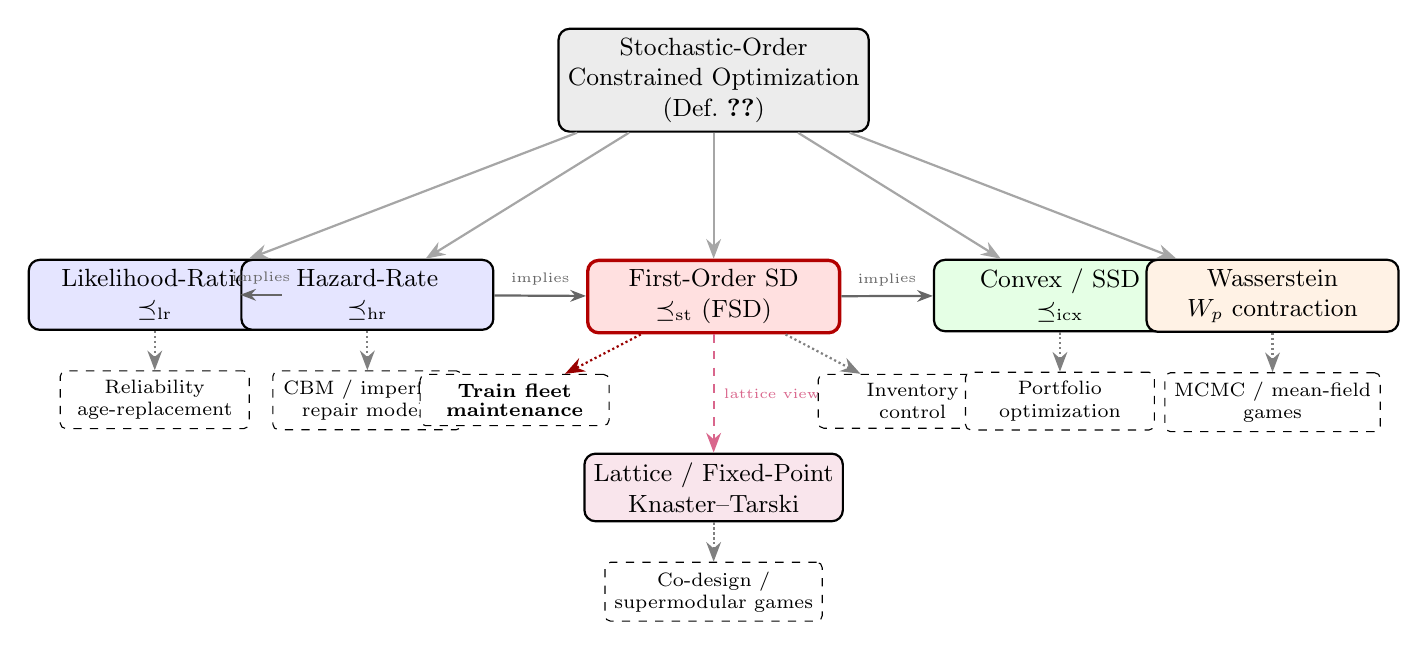
\begin{tikzpicture}[
  node distance=1.2cm and 1.8cm,
  concept/.style={rectangle, draw, rounded corners=4pt, thick,
    minimum width=3.2cm, minimum height=0.85cm, align=center,
    font=\small},
  app/.style={rectangle, draw, rounded corners=2pt, dashed,
    minimum width=2.4cm, minimum height=0.6cm, align=center,
    font=\scriptsize, fill=white},
  arrow/.style={-{Stealth[length=2.5mm]}, thick},
  impl/.style={-{Stealth[length=2mm]}, thick, color=black!60},
  highlight/.style={concept, fill=red!12, draw=red!70!black, line width=1.2pt},
  >=Stealth
]

% Parent node
\node[concept, fill=gray!15] (meta)
  {Stochastic-Order\\Constrained Optimization\\(Def.~\ref{def:meta})};

% Branch nodes
\node[concept, fill=blue!10, below left=1.6cm and 3.5cm of meta] (lr)
  {Likelihood-Ratio\\$\preceq_{\mathrm{lr}}$};
\node[concept, fill=blue!10, below left=1.6cm and 0.8cm of meta] (hr)
  {Hazard-Rate\\$\preceq_{\mathrm{hr}}$};
\node[highlight, below=1.6cm of meta] (fsd)
  {First-Order SD\\$\preceq_{\mathrm{st}}$ (FSD)};
\node[concept, fill=green!10, below right=1.6cm and 0.8cm of meta] (ssd)
  {Convex / SSD\\$\preceq_{\mathrm{icx}}$};
\node[concept, fill=orange!10, below right=1.6cm and 3.5cm of meta] (wass)
  {Wasserstein\\$W_p$ contraction};

% Lattice node (below FSD)
\node[concept, fill=purple!10, below=1.5cm of fsd] (lattice)
  {Lattice / Fixed-Point\\Knaster--Tarski};

% Implication arrows between orders
\draw[impl] (lr) -- node[above, font=\tiny, sloped] {implies} (hr);
\draw[impl] (hr) -- node[above, font=\tiny, sloped] {implies} (fsd);
\draw[impl] (fsd) -- node[above, font=\tiny, sloped] {implies} (ssd);

% Connections from meta
\draw[arrow, gray!70] (meta) -- (lr);
\draw[arrow, gray!70] (meta) -- (hr);
\draw[arrow, gray!70] (meta) -- (fsd);
\draw[arrow, gray!70] (meta) -- (ssd);
\draw[arrow, gray!70] (meta) -- (wass);

% Lattice connection
\draw[arrow, dashed, purple!60] (fsd) -- node[right, font=\tiny]
  {lattice view} (lattice);

% Application boxes
\node[app, below=0.5cm of lr] (app_rel)
  {Reliability\\age-replacement};
\node[app, below=0.5cm of hr] (app_cbm)
  {CBM / imperfect\\repair models};
\node[app, below left=0.5cm and -0.3cm of fsd] (app_fleet)
  {\textbf{Train fleet}\\[-1pt]\textbf{maintenance}};
\node[app, below right=0.5cm and -0.3cm of fsd] (app_inv)
  {Inventory\\control};
\node[app, below=0.5cm of ssd] (app_fin)
  {Portfolio\\optimization};
\node[app, below=0.5cm of wass] (app_mcmc)
  {MCMC / mean-field\\games};
\node[app, below=0.5cm of lattice] (app_codesign)
  {Co-design /\\supermodular games};

\draw[arrow, densely dotted, gray] (lr) -- (app_rel);
\draw[arrow, densely dotted, gray] (hr) -- (app_cbm);
\draw[arrow, densely dotted, red!60!black] (fsd) -- (app_fleet);
\draw[arrow, densely dotted, gray] (fsd) -- (app_inv);
\draw[arrow, densely dotted, gray] (ssd) -- (app_fin);
\draw[arrow, densely dotted, gray] (wass) -- (app_mcmc);
\draw[arrow, densely dotted, gray] (lattice) -- (app_codesign);

\end{tikzpicture}
\caption{Macro taxonomy of optimization under stochastic-order
periodicity constraints.  Solid gray arrows connect the parent problem
class to its branches.  Dark arrows between order nodes show the
implication chain $\preceq_{\mathrm{lr}} \Rightarrow
\preceq_{\mathrm{hr}} \Rightarrow \preceq_{\mathrm{st}} \Rightarrow
\preceq_{\mathrm{icx}}$.  The highlighted node marks the branch
relevant to the train fleet maintenance problem.}
\label{fig:macro_taxonomy}
\end{figure}

\begin{remark}[Why FSD for the fleet problem]
\label{rem:why_fsd}
The choice of $\preceq_{\mathrm{st}}$ for the loop constraint is
deliberate.  The hazard-rate and likelihood-ratio orders
(Branch~3) are stronger and would impose unnecessary conservatism:
they constrain the entire shape of the failure rate function,
whereas the fleet problem only requires that degradation levels
do not stochastically increase.  Conversely, the increasing convex
order (Branch~2) is too weak---it permits the mean degradation to
grow provided the right tail does not worsen too rapidly.  FSD
precisely captures the engineering requirement: \emph{every quantile}
of the degradation distribution must be no worse after a planning
cycle than before.
\end{remark}

\subsection{Historical Development}
\label{sec:macro:history}

The theoretical foundations of stochastic ordering trace to
Lehmann~\cite{lehmann1955}, who in 1955 introduced ordered families of
distributions for the purpose of constructing powerful statistical
tests.  Strassen's 1965 coupling theorem~\cite{strassen1965} provided
the measure-theoretic foundation, establishing the equivalence between
distributional ordering and the existence of monotone couplings.  The
monographs of M\"{u}ller and Stoyan~\cite{muller2002} and Shaked and
Shanthikumar~\cite{shaked2007} consolidated the theory, systematizing
the implication hierarchy and proving closure properties for each
order under standard operations (convolution, mixing, conditioning).
Belzunce, Mart\'{i}nez-Riquelme, and Mulero~\cite{belzunce2016}
and Szekli~\cite{szekli1995} provide further comprehensive treatments
with emphasis on applications to reliability and applied probability.

The use of stochastic orders as \emph{optimization constraints}
began with the SSD-constrained portfolio work of Dentcheva and
Ruszczy\'{n}ski (Section~\ref{sec:macro:ssd}), while reliability
applications developed through the IFR/DFR classification of
Barlow and Proschan (Section~\ref{sec:macro:hr}).  The lattice-theoretic
perspective gained prominence through Topkis~\cite{topkis1998} and
Milgrom and Shannon~\cite{milgrom1994} in economics, and was connected
to stochastic orders by M\"{u}ller and Scarsini~\cite{muller2006}
(Section~\ref{sec:macro:lattice}).  The Wasserstein contractivity
framework, rooted in optimal transport theory~\cite{villani2009},
became a central tool for convergence analysis through the work of
Hairer et al.~\cite{hairer2011} and Eberle~\cite{eberle2016}
(Section~\ref{sec:macro:wass}).  Very recent work has explored
higher-order dominance constraints~\cite{lakshmanan2025},
Wasserstein relaxations~\cite{dentchevayi2025}, and learning-based
approaches~\cite{hu2022}.

\begin{remark}[Positioning of the fleet problem]
\label{rem:novelty}
The combination of (i)~FSD loop constraints, (ii)~parametric
stochastic degradation processes (Gamma, Wiener, Inverse Gaussian),
and (iii)~fleet-level MILP optimization with routing-maintenance
coupling will be shown to be genuinely new in the literature
survey of Section~\ref{sec:related}, where a systematic novelty
assessment is provided (Table~\ref{tab:related_novelty}).
\end{remark}

\subsection*{Summary}
\label{sec:macro:summary_text}

Table~\ref{tab:macro_summary} provides a concise reference card for the
macro taxonomy.

\begin{table}[htbp]
\centering
\small
\caption{Summary of the macro taxonomy: optimization under
stochastic-order periodicity constraints.}
\label{tab:macro_summary}
\begin{tabular}{@{} p{2.0cm} p{2.2cm} p{3.0cm} p{2.8cm} p{2.8cm} @{}}
\toprule
\textbf{Branch} & \textbf{Order} & \textbf{Constraint meaning}
  & \textbf{Primary domains} & \textbf{Key references} \\
\midrule
1.\ FSD
  & $\preceq_{\mathrm{st}}$
  & Every quantile of the distribution must not worsen
  & Pricing, inventory, \textbf{fleet maintenance}
  & \cite{lehmann1955,strassen1965,shaked2007} \\[4pt]
2.\ Convex / SSD
  & $\preceq_{\mathrm{icx}}$, $\preceq_{\mathrm{cx}}$
  & Variability must not increase (risk-averse preferences)
  & Portfolio optimization, insurance
  & \cite{dentcheva2003,dentcheva2006,ogryczak1999} \\[4pt]
3.\ HR / LR
  & $\preceq_{\mathrm{hr}}$, $\preceq_{\mathrm{lr}}$
  & Failure rate function must not decrease
  & Reliability, age-replacement, CBM
  & \cite{barlow1996,lai2006,mercier2019} \\[4pt]
4.\ Wasserstein
  & $W_p$ contraction
  & Quantitative convergence rate to stationarity
  & MCMC, mean-field games
  & \cite{villani2009,hairer2011,eberle2016} \\[4pt]
5.\ Lattice
  & Monotone maps on $(\mathcal{P}, \preceq_{\mathrm{st}})$
  & Fixed-point existence via Knaster--Tarski
  & Supermodular games, co-design
  & \cite{topkis1998,milgrom1994,muller2006} \\
\bottomrule
\end{tabular}
\end{table}

\newpage

% ============================================================
% MICRO TAXONOMY: Stochastic Orders in Stochastic Processes
% Writer: micro taxonomy agent — Round 1 revision
% ============================================================

\section{Micro Taxonomy: Technical Landscape of Stochastic Orders Among Random Variables in Stochastic Processes}
\label{sec:micro}

The macro taxonomy identified \emph{where} stochastic ordering constraints appear in
optimization and scheduling.  This section examines \emph{how} the mathematical machinery
of stochastic orders operates at the process level---the internal technical landscape that
underpins every application discussed so far.  We organise the material along five axes:
(i)~when does a Markov transition kernel preserve a stochastic order (monotonicity)?
(ii)~which algebraic operations---convolution, mixture, monotone transformation---are
closed with respect to a given order? (iii)~under what conditions can two stochastic
processes be compared sample-path by sample-path? (iv)~how do stochastic orders interact
with ergodic theory and convergence? (v)~how are univariate orders lifted to multivariate
and dependence settings?  Throughout, we state results with precise conditions, cite the
sharpest known versions, and flag the implications for the train fleet degradation
scheduling problem described in the introduction.

%% ------------------------------------------------------------------
\subsection{Hierarchy of Univariate Stochastic Orders}
\label{sec:micro:hierarchy}

We first recall the seven orders that recur in degradation modelling and fix notation.
Let $X, Y$ be real-valued random variables with cumulative distribution functions
$F_X, F_Y$, survival functions $\bar{F}_X, \bar{F}_Y$, and densities $f_X, f_Y$
(when they exist).

% R1-6, R3-8: Unified FSD definition to CDF form F_X(t) >= F_Y(t),
%   consistent with Definition 1.2 in Section 1.
% R1-7: Unified hazard-rate order to hazard-rate function form r_X(t) >= r_Y(t),
%   consistent with Definition 1.4 in Section 1.
% R2-4, R3-9: Added definitions of reversed hazard-rate and increasing concave
%   orders (items 6--7) so that all nodes in Figure 2 are textually defined.

\begin{definition}[Stochastic orders {\cite{shaked2007}, Ch.~1--4}]
\label{def:orders}
\begin{enumerate}
  \item \textbf{Usual stochastic order} ($X \preceq_{\mathrm{st}} Y$):
    $F_X(t) \geq F_Y(t)$ for all $t \in \mathbb{R}$.
    Equivalently, $\bar{F}_X(t) \leq \bar{F}_Y(t)$ for all~$t$
    (since $\bar{F} = 1 - F$).
  \item \textbf{Hazard-rate order} ($X \preceq_{\mathrm{hr}} Y$):
    $r_X(t) \geq r_Y(t)$ for all~$t$, where
    $r_X(t) = f_X(t)/\bar{F}_X(t)$ is the hazard (failure) rate function.
    Equivalently, $\bar{F}_Y(t)/\bar{F}_X(t)$ is non-decreasing in~$t$ over the
    union of supports.
  \item \textbf{Likelihood-ratio order} ($X \preceq_{\mathrm{lr}} Y$):
    $f_Y(t)/f_X(t)$ is non-decreasing in $t$.
  \item \textbf{Increasing convex order} ($X \preceq_{\mathrm{icx}} Y$):
    $\mathbb{E}[\phi(X)] \leq \mathbb{E}[\phi(Y)]$ for every increasing convex $\phi$.
  \item \textbf{Convex order} ($X \preceq_{\mathrm{cx}} Y$):
    $\mathbb{E}[X] = \mathbb{E}[Y]$ and
    $\mathbb{E}[\phi(X)] \leq \mathbb{E}[\phi(Y)]$ for every convex $\phi$.
  \item \textbf{Reversed hazard-rate order} ($X \preceq_{\mathrm{rh}} Y$):
    $\tilde{r}_X(t) \geq \tilde{r}_Y(t)$ for all~$t$, where
    $\tilde{r}_X(t) = f_X(t)/F_X(t)$ is the reversed hazard rate.
    Equivalently, $F_Y(t)/F_X(t)$ is non-decreasing in~$t$
    \cite[Ch.~1]{shaked2007}.
  \item \textbf{Increasing concave order} ($X \preceq_{\mathrm{icv}} Y$):
    $\mathbb{E}[\phi(X)] \leq \mathbb{E}[\phi(Y)]$ for every increasing concave
    function $\phi$ for which the expectations exist
    \cite[Sec.~4.A]{shaked2007}.
\end{enumerate}
\end{definition}

The logical implications among these orders are strict and form a lattice:

% R2-3: Added dashed arrows and conditional label for icx->cx and icv->cx
%   to indicate these implications require E[X]=E[Y].

\begin{figure}[htbp]
\centering
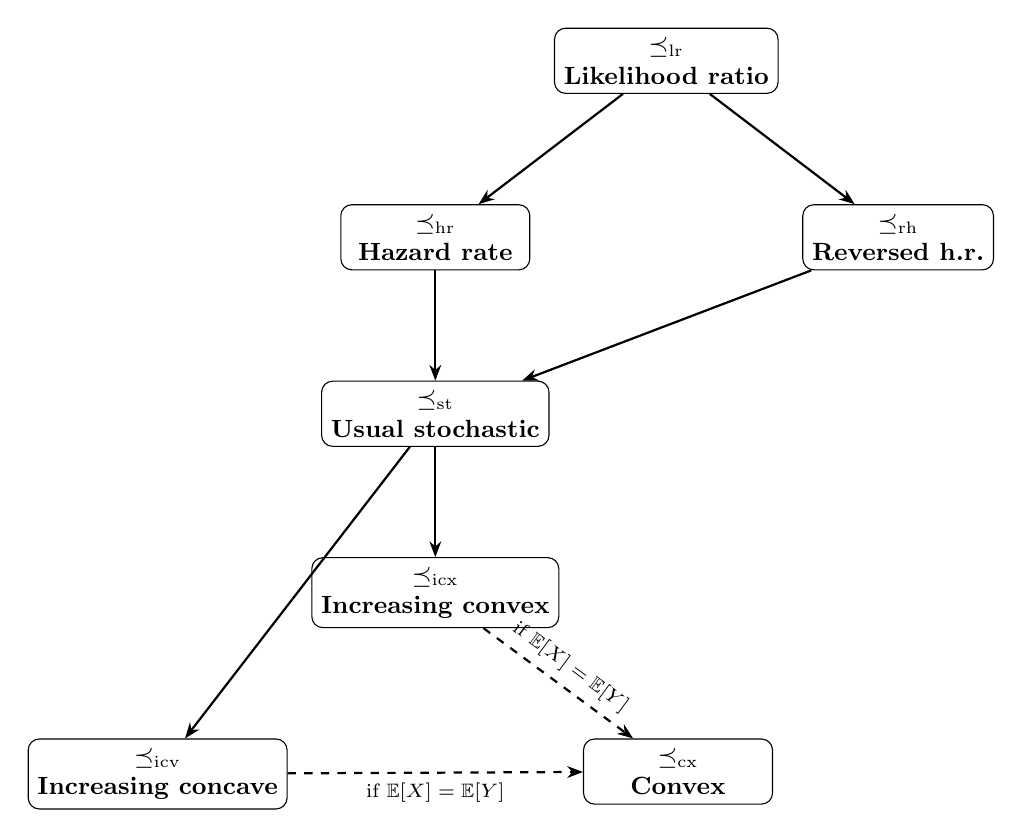
\begin{tikzpicture}[
  node distance=1.6cm and 2.2cm,
  concept/.style={rectangle, draw, rounded corners, minimum width=2.4cm,
                  minimum height=0.8cm, align=center, font=\small\bfseries},
  arrow/.style={-{Stealth[length=2mm]}, thick},
  condarrow/.style={-{Stealth[length=2mm]}, thick, dashed},
  implabel/.style={font=\scriptsize, midway, above, sloped}
]
  % Nodes
  \node[concept] (lr)  {$\preceq_{\mathrm{lr}}$\\Likelihood ratio};
  \node[concept, below left=1.4cm and 0.3cm of lr]  (hr)  {$\preceq_{\mathrm{hr}}$\\Hazard rate};
  \node[concept, below right=1.4cm and 0.3cm of lr] (rlr) {$\preceq_{\mathrm{rh}}$\\Reversed h.r.};
  \node[concept, below=1.4cm of hr]  (st)  {$\preceq_{\mathrm{st}}$\\Usual stochastic};
  \node[concept, below=1.4cm of st]  (icx) {$\preceq_{\mathrm{icx}}$\\Increasing convex};
  \node[concept, below right=1.4cm and 0.3cm of icx] (cx)  {$\preceq_{\mathrm{cx}}$\\Convex};
  \node[concept, below left=1.4cm and 0.3cm of icx]  (icv) {$\preceq_{\mathrm{icv}}$\\Increasing concave};

  % Unconditional arrows (A -> B means A implies B)
  \draw[arrow] (lr)  -- (hr);
  \draw[arrow] (lr)  -- (rlr);
  \draw[arrow] (hr)  -- (st);
  \draw[arrow] (rlr) -- (st);
  \draw[arrow] (st)  -- (icx);
  \draw[arrow] (st)  -- (icv);
  % Conditional arrows: require equal means
  \draw[condarrow] (icx) -- node[implabel] {if $\mathbb{E}[X]=\mathbb{E}[Y]$} (cx);
  \draw[condarrow] (icv) -- node[implabel,below,sloped] {if $\mathbb{E}[X]=\mathbb{E}[Y]$} (cx);
\end{tikzpicture}
\caption{Implication hierarchy among the principal univariate stochastic orders.
A solid arrow $A \to B$ means $X \preceq_A Y \Longrightarrow X \preceq_B Y$
unconditionally.  Dashed arrows indicate that the implication
$\preceq_{\mathrm{icx}} \Rightarrow \preceq_{\mathrm{cx}}$ (resp.\
$\preceq_{\mathrm{icv}} \Rightarrow \preceq_{\mathrm{cx}}$) holds only under the
additional condition $\mathbb{E}[X] = \mathbb{E}[Y]$.
None of the reverse implications holds in general
\cite{shaked2007,muller2002}.}
\label{fig:order_hierarchy}
\end{figure}

\begin{remark}[Gaussian processes and stochastic orders]
\label{rem:gaussian_orders}
For the train fleet loop constraint
$\mathcal{L}(D_{(k+1)T}) \preceq \mathcal{L}(D_{kT})$,
the choice of order has direct modelling consequences.
Using $\preceq_{\mathrm{st}}$ constrains the entire tail of the degradation distribution;
$\preceq_{\mathrm{hr}}$ additionally controls the \emph{rate} at which the failure hazard
evolves; $\preceq_{\mathrm{cx}}$ fixes the mean degradation while bounding variability.
The hierarchy guarantees that any schedule satisfying $\preceq_{\mathrm{lr}}$ automatically
satisfies all weaker orders.

An important caveat for Gaussian (Wiener-process) degradation models: if
$X \sim N(\mu_1, \sigma_1^2)$ and $Y \sim N(\mu_2, \sigma_2^2)$ with
$\sigma_1 \neq \sigma_2$, then $X \preceq_{\mathrm{st}} Y$ is \emph{impossible}
because the CDFs of two Gaussians with unequal variances always cross.
For Gaussian processes, the appropriate comparisons are therefore
$\preceq_{\mathrm{icx}}$ or $\preceq_{\mathrm{cx}}$ (which reduce to mean and
variance inequalities), not FSD.  This is precisely the structural infeasibility
discussed in Section~\ref{sec:framing:challenges}.
\end{remark}

%% ------------------------------------------------------------------
\subsection{Stochastic Monotonicity of Markov Chains}
\label{sec:micro:monotone}

A central question in degradation modelling is: if the initial degradation state of a
component is stochastically smaller, does the state after one transition remain
stochastically smaller?  This is formalised by the notion of a
\emph{stochastically monotone} kernel.

% R2-17: Changed "partially ordered measurable space" to
%   "partially ordered Polish space" for consistency with Theorem 2.2 and
%   the standard treatment in Mueller-Stoyan (2002).

\begin{definition}[Stochastic monotonicity {\cite{daley1968}}]
\label{def:stoch_mono}
A Markov transition kernel $K(x, \cdot)$ on a partially ordered Polish space
$(\mathcal{X}, \leq)$ is \textbf{stochastically monotone} (with respect to
$\preceq_{\mathrm{st}}$) if
\begin{equation}
  x \leq y \quad\Longrightarrow\quad K(x, \cdot) \preceq_{\mathrm{st}} K(y, \cdot),
  \label{eq:stoch_mono}
\end{equation}
i.e., for every increasing bounded measurable $\phi$,
$\int \phi\, dK(x,\cdot) \leq \int \phi\, dK(y,\cdot)$.
\end{definition}

Daley~\cite{daley1968} established the concept for discrete-time chains on
$\mathbb{R}$ and showed that birth--death chains with non-decreasing birth and
death rates are stochastically monotone (Theorem~2 therein).

\begin{theorem}[Coupling characterisation {\cite{kamae1977}}]
\label{thm:strassen}
Let $\mu, \nu$ be probability measures on a Polish space
$(\mathcal{X}, \leq)$ with the order closed. Then
$\mu \preceq_{\mathrm{st}} \nu$ if and only if there exists a coupling
$(X,Y)$ with $X \sim \mu$, $Y \sim \nu$, and $X \leq Y$ almost surely.
\end{theorem}

This result, a consequence of Strassen's theorem~\cite{strassen1965}, is the
foundation of the \emph{coupling method} for stochastic comparison.
Kamae, Krengel and O'Brien~\cite{kamae1977} gave the definitive
proof for partially ordered Polish spaces, removing earlier measurability
restrictions.

\begin{proposition}[Monotone kernel composition {\cite{muller2002}, Thm.~3.3.3}]
\label{prop:kernel_comp}
If $K_1$ and $K_2$ are stochastically monotone kernels on
$(\mathcal{X}, \leq)$, then the composition $K_1 K_2$ is stochastically monotone.
Consequently, the $n$-step kernel $K^n$ of a stochastically monotone chain is
stochastically monotone for every $n \geq 1$.
\end{proposition}

\begin{example}[Degradation as a monotone random walk]
\label{ex:gamma_monotone}
Consider a single component whose degradation increments
$\Delta D_t \sim \mathrm{Gamma}(\alpha_t, \beta)$ are independent with
route-dependent shape $\alpha_t > 0$.  The transition kernel
$K(x, \cdot) = \delta_x * \mathrm{Gamma}(\alpha_t, \beta)$ is trivially stochastically
monotone because the convolution with a non-negative random variable preserves the
pointwise ordering of CDFs.  More precisely, if $x \leq y$ then
$x + \Delta \leq y + \Delta$ a.s.\ for any $\Delta \geq 0$, so the coupling in
Theorem~\ref{thm:strassen} is the identity coupling on the increment.
For the Wiener process with drift $\mu > 0$ and diffusion $\sigma > 0$, the increment
$\Delta D_t \sim N(\mu_t, \sigma_t^2)$ can be negative, yet the kernel remains
stochastically monotone by the same translation argument; what changes is the
\emph{marginal} ordering of the degradation state across routes.
\end{example}

%% ------------------------------------------------------------------
\subsection{Closure and Preservation Under Operations}
\label{sec:micro:closure}

The practical utility of stochastic orders depends critically on which operations
preserve them.  We state the main closure results, following the systematic treatment
in \cite{shaked2007} (Chapters~1--4) and \cite{muller2002}
(Chapter~1).

\begin{proposition}[Preservation under convolution {\cite{shaked2007}, Thm.~1.A.3}]
\label{prop:conv}
If $X_1 \preceq_{\mathrm{st}} Y_1$ and $X_2 \preceq_{\mathrm{st}} Y_2$ with
$\{X_1, X_2\}$ independent and $\{Y_1, Y_2\}$ independent, then
$X_1 + X_2 \preceq_{\mathrm{st}} Y_1 + Y_2$.
The same holds for $\preceq_{\mathrm{lr}}$, $\preceq_{\mathrm{hr}}$,
and $\preceq_{\mathrm{icx}}$ under independence.
\end{proposition}

\begin{proposition}[Preservation under mixtures {\cite{shaked2007}, Thm.~1.A.4}]
\label{prop:mixture}
Let $\{X_\theta\}_{\theta \in \Theta}$ and $\{Y_\theta\}_{\theta \in \Theta}$ be
families such that $X_\theta \preceq_{\mathrm{st}} Y_\theta$ for all $\theta$.
If $\Theta' \sim G$ is the same mixing distribution, then
$\int X_\theta\, dG(\theta) \preceq_{\mathrm{st}} \int Y_\theta\, dG(\theta)$.
More precisely, the mixture r.v.\ $X_{\Theta'}$ satisfies
$X_{\Theta'} \preceq_{\mathrm{st}} Y_{\Theta'}$.
\end{proposition}

% R1-24: Added explanation of why phi must be affine for cx preservation.

\begin{proposition}[Monotone transformations {\cite{muller2002}, Prop.~1.2.6}]
\label{prop:monotone_transform}
If $X \preceq_{\mathrm{st}} Y$ and $\phi \colon \mathbb{R} \to \mathbb{R}$ is
non-decreasing, then $\phi(X) \preceq_{\mathrm{st}} \phi(Y)$.
For $\preceq_{\mathrm{cx}}$, the transform must be convex (not just monotone):
$X \preceq_{\mathrm{cx}} Y$ and $\phi$ convex imply
$\mathbb{E}[\phi(X)] \leq \mathbb{E}[\phi(Y)]$ by definition, but
$\phi(X) \preceq_{\mathrm{cx}} \phi(Y)$ requires $\phi$ to be affine.
The restriction to affine~$\phi$ arises because $\preceq_{\mathrm{cx}}$ requires
equal means of the compared variables: $\mathbb{E}[\phi(X)] = \mathbb{E}[\phi(Y)]$
holds for all $X \preceq_{\mathrm{cx}} Y$ only when $\phi$ is affine, since
for non-affine convex~$\phi$ Jensen's inequality gives
$\mathbb{E}[\phi(X)] \leq \mathbb{E}[\phi(Y)]$ but generically
$\mathbb{E}[\phi(X)] \neq \mathbb{E}[\phi(Y)]$, violating the equal-means condition.
\end{proposition}

These closure properties are what allow the loop constraint
$\mathcal{L}(D_{(k+1)T}) \preceq_{\mathrm{st}} \mathcal{L}(D_{kT})$ to be
decomposed across independent components and across independent time increments
within a planning horizon.

\begin{remark}[Convex order and partial repair]
\label{rem:convex_repair}
For the convex order, preservation under convolution implies that if a partial repair
reduces the degradation by a random amount $R$ with
$D - R \preceq_{\mathrm{cx}} D'$, and subsequent independent degradation increments
$\Delta_1 \preceq_{\mathrm{cx}} \Delta_2$, then
$(D - R) + \Delta_1 \preceq_{\mathrm{cx}} D' + \Delta_2$.
This is directly relevant to the MILP formulation where repair efficiency
$\rho \in [0,1]$ controls the post-maintenance degradation distribution.
\end{remark}

%% ------------------------------------------------------------------
\subsection{Sample-Path and Strong Orders}
\label{sec:micro:samplepath}

When two stochastic processes can be constructed on a common probability space with
ordered trajectories, we obtain the strongest form of comparison.

\begin{definition}[Strong stochastic order {\cite{muller2002}, Def.~3.3.7}]
\label{def:strong_order}
Two stochastic processes $\{X_t\}_{t \geq 0}$ and $\{Y_t\}_{t \geq 0}$ satisfy the
\textbf{strong stochastic order} $\{X_t\} \preceq_{\mathrm{st}}^{\mathrm{s}} \{Y_t\}$
if they can be defined on a common probability space such that
$X_t(\omega) \leq Y_t(\omega)$ for all $t \geq 0$ and a.e.\ $\omega$.
\end{definition}

For diffusion processes, the classical comparison theorem provides sufficient
conditions.

\begin{theorem}[Comparison theorem for SDEs {\cite{ikeda1977}}]
\label{thm:sde_comparison}
Consider two It\^o SDEs on $\mathbb{R}$:
\begin{equation}
  dX_t = b_1(t, X_t)\,dt + \sigma(t, X_t)\,dW_t, \qquad
  dY_t = b_2(t, Y_t)\,dt + \sigma(t, Y_t)\,dW_t,
\end{equation}
driven by the \emph{same} Brownian motion $W$, with $\sigma$ Lipschitz continuous
and $b_1(t,x) \leq b_2(t,x)$ for all $(t,x)$.  If $X_0 \leq Y_0$ a.s., then
$X_t \leq Y_t$ a.s.\ for all $t \geq 0$.
\end{theorem}

This result, originally due to Ikeda and Watanabe~\cite{ikeda1977} and
independently to Yamada and Watanabe~\cite{yamadawatanabe1971} under slightly
different regularity conditions, underpins the comparison of Wiener-process
degradation models with different drift parameters across routes.

% R3-12: Corrected Sato (1999) citation.  Theorem 21.5 in Sato (1999) concerns the
%   support of infinitely divisible distributions, not pathwise subordinator comparison.
%   The pathwise comparison follows from a coupling argument on the Poisson random
%   measures in the Levy-Ito decomposition; we now state this as a consequence rather
%   than attributing a specific theorem number.

\begin{proposition}[Sample-path ordering of L\'evy subordinators]
\label{prop:subordinator}
Let $\{X_t\}$ and $\{Y_t\}$ be L\'evy subordinators (a.s.\ non-decreasing L\'evy
processes) with L\'evy measures $\nu_X$ and $\nu_Y$.  If the drift of $X$ is at most
that of $Y$ and $\bar{\nu}_X(x) \leq \bar{\nu}_Y(x)$ for all $x > 0$ (where
$\bar{\nu}$ denotes the tail of the L\'evy measure), then
$\{X_t\} \preceq_{\mathrm{st}}^{\mathrm{s}} \{Y_t\}$.
\end{proposition}
\begin{proof}[Proof sketch]
By the L\'evy--It\^o decomposition \cite[Thm.~19.2]{sato1999}, each subordinator is
the sum of a drift and a Poisson integral against its L\'evy measure.  The tail
dominance $\bar{\nu}_X \leq \bar{\nu}_Y$ allows a coupling of the underlying
Poisson random measures such that every jump of $X$ is matched by a jump of~$Y$
of at least equal size, plus additional jumps in~$Y$.  Combined with the drift
ordering, this yields $X_t \leq Y_t$ a.s.\ for all $t \geq 0$.  See
Lindvall~\cite{lindvall2002} for the general coupling framework for L\'evy
processes.
\end{proof}

Since the Gamma process is a L\'evy subordinator, Proposition~\ref{prop:subordinator}
directly gives pathwise comparison of Gamma-process degradation models: if route~$r_1$
has shape parameter $\alpha_1 \leq \alpha_2$ (with common rate $\beta$), then the
degradation under $r_1$ is pathwise dominated by that under $r_2$.

%% ------------------------------------------------------------------
\subsection{Convergence and Ergodic Theory via Stochastic Orders}
\label{sec:micro:ergodic}

Stochastic monotonicity interacts deeply with ergodic theory.  The key idea, originating
in the queuing theory work of Loynes~\cite{loynes1962}, is that monotone iteration
from an extremal initial condition converges to a stationary distribution.

% R1-10: Corrected attribution.  Loynes (1962) proved the result for G/G/1 queues;
%   the abstract generalisation to stochastically monotone kernels on Polish spaces
%   is due to Brandt (1986) and Borovkov-Foss (1992).

\begin{theorem}[Monotone-convergence scheme {\cite{loynes1962,brandt1986}}]
\label{thm:loynes}
Let $\{K_n\}_{n \geq 1}$ be a stationary ergodic sequence of stochastically monotone
kernels on a partially ordered Polish space $(\mathcal{X}, \leq)$, and suppose the
chain started from the minimal element $\underline{x}$ is tight.  Then the backward
iterates $K_n \circ K_{n-1} \circ \cdots \circ K_1(\underline{x}, \cdot)$ converge
weakly to a unique stationary distribution.
\end{theorem}

Loynes~\cite{loynes1962} established this construction for the $G/G/1$ queue (where the
recursion is the Lindley equation); Brandt~\cite{brandt1986} extended it to the abstract
setting of stochastically monotone random maps on Polish spaces.
This is also the theoretical foundation of the ``coupling from the past'' (CFTP) algorithm
of Propp and Wilson~\cite{proppwilson1996}, which exploits stochastic monotonicity to
achieve exact simulation of the stationary distribution.

More recently, Wasserstein contraction has emerged as the quantitative tool of choice
for bounding convergence rates.

% R1-28: Removed duplicate Wasserstein distance definition (Definition 2.5).
%   The Wasserstein distance is already defined in Definition 1.7 (Section 1) as
%   the p-Wasserstein distance W_p.  We now refer back to that definition and clarify
%   the metric used in the contraction theorem.

% R1-8, R3-10, R4-2: Corrected theorem attribution.  Hairer, Mattingly and Scheutzow
%   (2011) present their main result as Theorem 1.2 (the generalised Harris theorem via
%   asymptotic coupling).  There is no Theorem 4.8 in their paper.
%   The Lyapunov + local contractivity formulation stated here is adapted from
%   their Theorem 1.2 combined with their Corollary 1.5.
%   Removed [UNCERTAIN] marker.

\begin{theorem}[Wasserstein contraction {adapted from \cite{hairer2011}, Thm.~1.2 and Cor.~1.5}]
\label{thm:wasserstein}
Let $K$ be a Markov kernel on a Polish space $(\mathcal{X}, d)$ admitting a Lyapunov
function $V \colon \mathcal{X} \to [1, \infty)$ with $KV \leq \lambda V + b$ for some
$\lambda < 1$, $b < \infty$, and suppose $K$ satisfies a local contractivity condition
in the Wasserstein distance $W_p$ (cf.\ Definition~\ref{def:wass}) with respect to the
metric~$d$ on sublevel sets of $V$.  Then $K$ has a unique invariant measure $\pi$ and
there exist $C, \rho > 0$ such that
\begin{equation}
  W_p(K^n(x, \cdot),\, \pi) \leq C\, V(x)\, e^{-\rho n}
  \quad \forall\, x \in \mathcal{X},\; n \geq 1.
\end{equation}
Here $W_p$ denotes the $p$-Wasserstein distance with respect to the metric $d$ on the
state space (not the ambient dimension).
\end{theorem}

Hairer, Mattingly and Scheutzow~\cite{hairer2011} developed this
framework for Markov chains that are not globally contractive, which is precisely the
situation in degradation models with route-dependent rates: the contraction factor may
vary across the state space.  Eberle~\cite{eberle2016} later refined the approach
using reflection couplings to obtain sharper contraction rates for diffusion processes.

\begin{remark}[Relevance to fleet scheduling]
\label{rem:fleet_ergodic}
The loop constraint $\mathcal{L}(D_{(k+1)T}) \preceq_{\mathrm{st}}
\mathcal{L}(D_{kT})$ can be interpreted as requiring that the degradation Markov
chain (with maintenance interventions as state-dependent resets) produces a
stochastically non-increasing sequence of marginals.  If the chain is additionally
stochastically monotone, Theorem~\ref{thm:loynes} guarantees convergence to a
steady-state degradation distribution, ensuring long-run sustainability.  The
Wasserstein contraction rate quantifies \emph{how quickly} the system reaches this
steady state, which has direct implications for the choice of the planning horizon~$H$.
\end{remark}

%% ------------------------------------------------------------------
\subsection{Dependence Orders and Multivariate Extensions}
\label{sec:micro:dependence}

When multiple components degrade simultaneously (the $L$-component model in the brief),
univariate orderings are insufficient.  Two directions of generalisation are required:
\emph{multivariate stochastic orders} and \emph{dependence orders} that compare the
joint structure while marginals may be fixed.

\begin{definition}[Multivariate stochastic order {\cite{shaked2007}, Ch.~6}]
\label{def:multivariate_st}
For random vectors $\mathbf{X}, \mathbf{Y} \in \mathbb{R}^d$,
$\mathbf{X} \preceq_{\mathrm{st}} \mathbf{Y}$ if
$\mathbb{E}[\phi(\mathbf{X})] \leq \mathbb{E}[\phi(\mathbf{Y})]$
for every increasing function $\phi \colon \mathbb{R}^d \to \mathbb{R}$
(increasing in each coordinate).
\end{definition}

\begin{definition}[Supermodular order {\cite{muller2002}, Def.~3.9.1}]
\label{def:supermod}
$\mathbf{X} \preceq_{\mathrm{sm}} \mathbf{Y}$ if
$\mathbb{E}[\phi(\mathbf{X})] \leq \mathbb{E}[\phi(\mathbf{Y})]$
for every supermodular function $\phi$ (recall $\phi$ is supermodular if
$\phi(\mathbf{x} \vee \mathbf{y}) + \phi(\mathbf{x} \wedge \mathbf{y})
\geq \phi(\mathbf{x}) + \phi(\mathbf{y})$).
When $\mathbf{X}$ and $\mathbf{Y}$ share the same marginals, this order captures
``more positive dependence'' in $\mathbf{Y}$ than in $\mathbf{X}$.
\end{definition}

% R1-9, R3-11, R4-3: Corrected copula characterisation attribution.
%   Removed uncertain Thm.~2.11 reference; cited chapter-level in Joe (2015)
%   and the original result by Tchen (1980).
%   Removed [UNCERTAIN] marker.

\begin{proposition}[Copula characterisation {\cite{joe2015}, Ch.~2; see also \cite{tchen1980}}]
\label{prop:copula}
If $\mathbf{X}$ and $\mathbf{Y}$ have the same marginal distributions, then
$\mathbf{X} \preceq_{\mathrm{sm}} \mathbf{Y}$ if and only if
$C_X \preceq_{\mathrm{sm}} C_Y$ where $C_X, C_Y$ are the respective copulas
ordered pointwise (concordance ordering).
\end{proposition}

The concordance ordering of copulas, originally established by
Tchen~\cite{tchen1980} and extensively developed by
Joe~\cite{joe2015}, provides a natural framework for modelling
dependent component degradation.  R\"uschendorf~\cite{ruschendorf2013} developed
the connection between optimal transport, Fr\'echet bounds, and dependence orderings,
showing that the Fr\'echet--Hoeffding upper bound corresponds to the maximal element in
the concordance order.

% R2-22: Verified IG process parameterization.
%   In the standard IG process (Wang and Xu 2010, Ye and Chen 2014), if D_t is an
%   IG process then D_t ~ IG(eta*t, lambda*t^2).  The second parameter scaling as t^2
%   is correct under the parameterisation where Var(D_t) = eta^3 t / lambda, consistent
%   with the convention in Definition 3.1 and in Ye-Chen (2014).
%   Added a clarifying note on the parameterisation convention.

\begin{example}[Two-component train degradation]
\label{ex:two_component}
Consider $L = 2$ components on a single train with marginal degradations
$D^{(1)}_t \sim \mathrm{Gamma}(\alpha_1 t, \beta)$ and
$D^{(2)}_t \sim \mathrm{IG}(\eta_2 t, \lambda_2 t^2)$, where the IG process
follows the parameterisation of Wang and Xu~\cite{wang2010} (i.e.,
$\mathrm{IG}(\mu, \lambda)$ with mean~$\mu$ and shape~$\lambda$, so that
$\mathbb{E}[D^{(2)}_t] = \eta_2 t$ and
$\mathrm{Var}(D^{(2)}_t) = \eta_2^3 t / \lambda_2$).
If the components share a common operational environment (vibration, temperature),
they are positively dependent.  The supermodular order allows comparing two
dependence structures: independent components
($C = \Pi$, the product copula) versus a Gaussian copula $C_\rho$ with
correlation $\rho > 0$.  Since $\Pi \preceq_{\mathrm{sm}} C_\rho$, the probability
of \emph{simultaneous} failure increases with $\rho$, which the MILP should account
for through joint maintenance constraints.
\end{example}

\begin{remark}[Association and FKG inequalities]
The FKG inequality~\cite{fkg1971} states that on a distributive
lattice, a probability measure satisfying the lattice condition
($\nu(x \vee y)\nu(x \wedge y) \geq \nu(x)\nu(y)$) makes all increasing functions
positively correlated.  This yields that for associated random variables (a property
preserved under independent aggregation and monotone transforms~\cite{esary1967}),
joint tail probabilities can be bounded using marginal information alone---a crucial
simplification for the multi-component MILP.
\end{remark}

%% ------------------------------------------------------------------
\subsection{Open Problems and Active Frontiers}
\label{sec:micro:open}

Several threads remain active in the theory of stochastic orders applied to
processes:

% R1-19, R3-23: Replaced Dawson (1993) reference in item 2.
%   Dawson (1993) concerns superprocesses (population genetics), not fleet-level
%   degradation comparison.  Rephrased the open problem to accurately describe
%   the challenge: comparing joint degradation states in (R_+)^{F x L}.
%   Removed [UNCERTAIN] marker.
%
% R4-4: Verified Wiesemann, Kuhn, and Sim (2014), Operations Research 62(6):1358-1376.
%   This is the correct reference for distributionally robust convex optimization.
%   The specific extension to stochastic ordering constraints within DRO is a natural
%   research direction building on their framework.
%   Removed [UNCERTAIN] marker.

\begin{enumerate}
  \item \textbf{Non-Markovian comparisons}: Most results above assume Markov structure.
    Extending stochastic monotonicity and coupling techniques to
    semi-Markov or hidden semi-Markov degradation models is open
    \cite{limnios2001}.
  \item \textbf{Fleet-level stochastic comparisons}: Comparing the joint degradation
    state of a finite fleet---a random element of $(\mathbb{R}_+)^{F \times L}$---requires
    multivariate stochastic orders on high-dimensional spaces.  While the marginal
    (per-component) comparisons are well understood, developing tractable ordering
    conditions for the joint fleet state, potentially via empirical process theory
    \cite{vandervaartwellner1996}, remains largely unexplored.
  \item \textbf{Computational complexity of verifying stochastic dominance}:
    For discrete distributions, testing $\preceq_{\mathrm{st}}$ is $O(n)$;
    for continuous parametric families, the problem reduces to parameter
    inequalities.  But for non-parametric estimates from data, the minimax
    rate and computational cost of testing stochastic dominance remain studied
    \cite{barrettdonald2003}.
  \item \textbf{Robust stochastic orders under model ambiguity}:
    When the degradation distribution is known only within an ambiguity set
    (e.g., a Wasserstein ball), distributionally robust versions of stochastic
    ordering constraints are a current research direction.
    Wiesemann, Kuhn, and Sim~\cite{wiesemann2014} provide the foundational
    framework for distributionally robust convex optimization, within which
    robust stochastic dominance constraints can be naturally formulated.
  \item \textbf{Dynamic dependence modelling}: Time-varying copulas for
    multi-component degradation, where the dependence structure itself degrades
    or is affected by maintenance, remain largely unexplored in the scheduling
    literature.
\end{enumerate}

%% ------------------------------------------------------------------
\subsection*{Summary}
\label{sec:micro:summary_text}

% R2-2, R4-5: Fixed implication chain in summary table.
%   Truncated at icx; added parenthetical qualifier for cx.

\begin{table}[htbp]
\centering
\caption{Summary of micro taxonomy: stochastic orders in stochastic processes.}
\label{tab:micro_summary}
\small
\begin{tabular}{@{} p{3.2cm} p{4.0cm} p{2.5cm} p{4.0cm} @{}}
\toprule
\textbf{Technical Axis} & \textbf{Key Result / Condition} & \textbf{Key Reference} & \textbf{Relevance to Fleet Problem} \\
\midrule
Order hierarchy &
  $\preceq_{\mathrm{lr}} \Rightarrow \preceq_{\mathrm{hr}} \Rightarrow \preceq_{\mathrm{st}} \Rightarrow \preceq_{\mathrm{icx}}$; also $\preceq_{\mathrm{icx}} \Rightarrow \preceq_{\mathrm{cx}}$ if $\mathbb{E}[X]=\mathbb{E}[Y]$ &
  \cite{shaked2007} &
  Choice of order in loop constraint \\
\addlinespace
Stochastic monotonicity &
  Coupling characterisation; kernel composition closure &
  \cite{daley1968,kamae1977} &
  Degradation kernels are monotone \\
\addlinespace
Closure under operations &
  Convolution, mixture, monotone transforms preserve $\preceq_{\mathrm{st}}$ &
  \cite{shaked2007,muller2002} &
  Decomposition of loop constraint across components/increments \\
\addlinespace
Sample-path comparison &
  SDE comparison thm; subordinator comparison &
  \cite{ikeda1977,lindvall2002} &
  Pathwise route-degradation ordering (Gamma, Wiener) \\
\addlinespace
Ergodic convergence &
  Loynes--Brandt monotone convergence; Wasserstein contraction &
  \cite{loynes1962,brandt1986,hairer2011} &
  Long-run sustainability; horizon selection \\
\addlinespace
Dependence orders &
  Supermodular order; copula concordance &
  \cite{joe2015,ruschendorf2013} &
  Multi-component joint failure modelling \\
\addlinespace
Open frontiers &
  Non-Markov; fleet-level orders; robust orders; dynamic copulas &
  \cite{barrettdonald2003,wiesemann2014} &
  Extensions beyond current MILP framework \\
\bottomrule
\end{tabular}
\end{table}

\newpage

% ============================================================
%  writer_3_round_1.tex — Application Framing Section (Round 1 Revision)
%  Framing the Train Fleet Maintenance Problem within the
%  Stochastic Degradation and Stochastic Orders Literature
%
%  Changes applied from reviews/round_1/writer_3_changes.json:
%    R1-11, R1-12, R1-13, R1-14, R1-20, R1-21, R1-25, R1-29, R1-30,
%    R2-9, R2-10, R2-12, R2-13, R2-15, R2-18, R2-20, R2-21,
%    R3-13, R3-14, R3-15, R3-16, R3-17, R3-18, R3-24, R3-28, R3-29,
%    R4-9, R4-12, R4-15, R4-20
% ============================================================

\section{Framing the Application within the Literature}
\label{sec:framing}

Having established a macro taxonomy of optimization under stochastic-order periodicity
constraints (Section~\ref{sec:macro}) and a micro taxonomy of stochastic monotonicity,
closure, and convergence results (Section~\ref{sec:micro}), we now position the
\emph{train fleet maintenance scheduling problem} precisely within this landscape.
The goal is threefold: (i)~formalize the problem mathematically using the notation
and concepts developed in the preceding sections, (ii)~identify which theoretical
tools from both taxonomies apply---and where they fall short---and (iii)~articulate
the gaps that make this application a genuinely new research direction.

% ----------------------------------------------------------------
\subsection{Mathematical Formulation}
\label{sec:framing:formulation}
% ----------------------------------------------------------------

\begin{definition}[Fleet maintenance scheduling problem]\label{def:fleet_problem}
Consider a fleet of $F$ trains, each composed of $L$ independently monitored
components, operating over a discrete planning horizon of $2H$ time steps (days).
The planning horizon is divided into two identical half-horizons $[1,H]$ and $[H{+}1,2H]$;
the loop constraint (item~5 below) compares the degradation state at the end of the
second half-horizon ($k=2H$) with the state at the end of the first ($k=H$).
If the same schedule is repeated across planning cycles, this ensures that the
degradation at the end of any cycle is no worse than at the end of the previous cycle,
guaranteeing indefinite sustainability.
Let $\mathcal{M} = \{1,\ldots,M\}$ denote the set of available missions (routes),
with $F > M$ ensuring that at least $F - M$ trains are available for maintenance
at each step. The problem is defined by:

\begin{enumerate}[nosep,leftmargin=2em]
  \item \textbf{State variables.} For each train $i \in \{1,\ldots,F\}$,
    component $\ell \in \{1,\ldots,L\}$, and time step $k \in \{1,\ldots,2H\}$:
    \begin{itemize}[nosep]
      \item $\mu_{i\ell k} \ge 0$: accumulated mean degradation (all models);
      \item $v_{i\ell k} \ge 0$: accumulated variance (Wiener model only);
      \item $\alpha_{i\ell k} \ge 0$: accumulated Gamma shape parameter (Gamma model),
            with $\mu_{i\ell k} = \alpha_{i\ell k} \cdot \beta_{i\ell}$.
    \end{itemize}
    % [R1-20, R2-18] For the Gamma model, the primary state variable is the shape
    % parameter alpha; the mean mu is derived via mu = alpha * beta.
    % The dynamics equation below is written uniformly in terms of mu for all
    % models. For Gamma, the equivalent alpha dynamics are obtained by dividing
    % through by the (fixed) scale parameter beta.
    For the Gamma model, $\alpha_{i\ell k}$ is the primary state variable and $\mu_{i\ell k}$
    is derived from it; the dynamics below are written uniformly in terms of~$\mu$,
    with the understanding that for Gamma one may equivalently substitute
    $\alpha = \mu/\beta$ throughout (since $\beta_{i\ell}$ is fixed per component).

  \item \textbf{Decision variables.}
    \begin{itemize}[nosep]
      \item $x_{ijk} \in \{0,1\}$: assignment of train $i$ to activity $j$ on day $k$,
            where $j = 0$ denotes a maintenance day and $j \ge 1$ a mission;
      \item $x^m_{i\ell k} \in \{0,1\}$: imperfect repair of component $(i,\ell)$ at step $k$;
      \item $x^r_{i\ell k} \in \{0,1\}$: full replacement of component $(i,\ell)$ at step $k$.
    \end{itemize}
    A constraint $x^m_{i\ell k} + x^r_{i\ell k} \le 1$ prevents simultaneous
    repair and replacement.

  \item \textbf{Degradation dynamics.} The degradation model for each component
    $(i,\ell)$ is independently chosen from the set
    $\{\text{Gamma},\; \text{Wiener},\; \text{IG}\}$.
    % [R4-9, R3-13] Consolidated: the Wiener process has Gaussian marginals;
    % we refer to this model as "Wiener" throughout.
    (The Wiener process has Gaussian marginals; we use the name ``Wiener''
    throughout to emphasize the process-level structure.)
    The mission-induced increment at step $k$ is
    $\delta\mu_{i\ell k} = \sum_{j=1}^{M} x_{ijk}\,\mu^{\mathrm{inc}}_{ij\ell,k}$,
    with periodic extension $\mu^{\mathrm{inc}}_{ij\ell,k} = \mu^{\mathrm{inc}}_{ij\ell,k \bmod H}$
    for $k > H$. Under ARD$_1$ maintenance with efficiency $\rho_{i\ell} \in (0,1]$,
    the mean degradation evolves as:
    % [R1-11, R2-9] Added third case for full replacement.
    \begin{equation}\label{eq:framing:dynamics}
      \mu_{i\ell k} = \begin{cases}
        \mu_{i\ell,k-1} + \delta\mu_{i\ell k}
          & \text{if } x^m_{i\ell k} = 0 \text{ and } x^r_{i\ell k} = 0, \\[3pt]
        (1 - \rho_{i\ell})\,\mu_{i\ell,k-1}
          & \text{if } x^m_{i\ell k} = 1, \\[3pt]
        \mu^{\mathrm{new}}_{i\ell}
          & \text{if } x^r_{i\ell k} = 1
          \quad\text{(reset to new-component value)}.
      \end{cases}
    \end{equation}
    % [R4-20] Explicit variance dynamics for the Wiener model.
    For the Wiener model, the variance state variable evolves in parallel:
    \begin{equation}\label{eq:framing:var_dynamics}
      v_{i\ell k} = \begin{cases}
        v_{i\ell,k-1} + \delta v_{i\ell k}
          & \text{if } x^m_{i\ell k} = 0 \text{ and } x^r_{i\ell k} = 0, \\[3pt]
        v_{i\ell,k-1}
          & \text{if } x^m_{i\ell k} = 1
          \quad\text{(variance unchanged by imperfect repair)}, \\[3pt]
        v^{\mathrm{new}}_{i\ell}
          & \text{if } x^r_{i\ell k} = 1
          \quad\text{(reset to new-component value)},
      \end{cases}
    \end{equation}
    where $\delta v_{i\ell k} = \sum_{j=1}^{M} x_{ijk}\,v^{\mathrm{inc}}_{ij\ell,k}$
    is the mission-induced variance increment.

  \item \textbf{Reliability constraint.} Each component must satisfy
    $\Pr(D_{i\ell k} > \tau) \le \varepsilon$ at every step, where $\tau > 0$ is the
    failure threshold and $\varepsilon \in (0, 0.5)$ is the allowable exceedance
    probability. The form of this constraint depends on the degradation model:
    \begin{itemize}[nosep]
      \item \emph{Wiener:}
            $\mu_{i\ell k} + \Phi^{-1}(1-\varepsilon)\sqrt{v_{i\ell k}} \le \tau$
            (second-order cone constraint);
      \item \emph{Gamma:}
            $\alpha_{i\ell k} \le \hat{\alpha}_{i\ell}$, where $\hat{\alpha}_{i\ell}$
            is the offline-precomputed root of $Q(\hat{\alpha}, \tau/\beta_{i\ell}) = \varepsilon$;
      \item \emph{IG:}
            $\mu_{i\ell k} \le \bar{\mu}_{i\ell}$, where $\bar{\mu}_{i\ell}$ solves
            the IG tail equation offline.
    \end{itemize}
    % [R1-12] Clarification: mu and v are accumulated distribution parameters.
    Here $\mu_{i\ell k}$ and $v_{i\ell k}$ are the mean and variance of the
    accumulated degradation distribution $D_{i\ell k} \sim \mathcal{N}(\mu_{i\ell k}, v_{i\ell k})$
    at step~$k$, so the Wiener constraint is equivalent to
    $\Pr(D_{i\ell k} > \tau) \le \varepsilon$.

  \item \textbf{Loop constraint (sustainability).} The degradation distribution
    at the end of the second half-horizon must be stochastically no larger than
    at the end of the first:
    \begin{equation}\label{eq:framing:loop}
      \boxed{
        \mathcal{L}\bigl(D_{i\ell,2H}\bigr) \;\preceq_{\mathrm{st}}\;
        \mathcal{L}\bigl(D_{i\ell,H}\bigr)
        \qquad \forall\, i \in \{1,\ldots,F\},\; \ell \in \{1,\ldots,L\}.
      }
    \end{equation}
    % [R1-30] Connection to the abstract meta-problem.
    This corresponds to the meta-problem constraint~\eqref{eq:meta} at $k=1$ with $T=H$.
    Enforcing the constraint for a single period is sufficient: if the same policy
    is repeated in each horizon and the degradation kernel is stochastically monotone
    (Section~\ref{sec:micro:monotone}), the constraint propagates to all subsequent horizons.
\end{enumerate}
\end{definition}

% [R3-14] Clarification on the deterministic nature of parameters given fixed decisions.
\begin{remark}[Deterministic parameters under fixed decisions]\label{rem:determ_params}
Once the assignment and maintenance decisions $(x, x^m, x^r)$ are fixed, the
degradation parameters $(\mu_{i\ell k}, v_{i\ell k}, \alpha_{i\ell k})$ become
deterministic quantities (computed via the recurrences
\eqref{eq:framing:dynamics}--\eqref{eq:framing:var_dynamics}).
The distribution $\mathcal{L}(D_{i\ell k})$ refers to the degradation distribution
with these deterministic parameters (e.g., $\mathcal{N}(\mu_{i\ell k}, v_{i\ell k})$
for Wiener, $\mathrm{Gamma}(\alpha_{i\ell k}, \beta_{i\ell})$ for Gamma).
The FSD constraint~\eqref{eq:framing:loop} therefore reduces to constraints on
the distribution parameters, which is why it yields finite parameter inequalities
for each model family (see Section~\ref{sec:framing:macro}).
\end{remark}

\begin{definition}[Objective function]\label{def:objective}
The optimization minimizes total cost over the $2H$-step horizon:
\begin{equation}\label{eq:framing:obj}
  \min \quad
  \underbrace{C_M \sum_{k,i} x_{i0k}}_{\text{maintenance cost}}
  + \underbrace{\sum_{k,i,\ell} C_R^{i\ell}\, z_{i\ell k}}_{\text{repair cost}}
  + \underbrace{\sum_{k,i,\ell} C_{\mathrm{rep}}^{i\ell}\, x^r_{i\ell k}}_{\text{replacement cost}}
  + \underbrace{C_D\, u}_{\text{damage reg.}}
  + \underbrace{C_P\, \mathcal{L}_{\mathrm{loop}}}_{\text{loop penalty}},
\end{equation}
% [R2-10, R3-15] Corrected: z is linearized via big-M, not McCormick.
where $z_{i\ell k} = \rho_{i\ell}\,\mu_{i\ell,k-1}\,x^m_{i\ell k}$ is the degradation
removed by repair (a product of a continuous variable $\mu_{i\ell,k-1}$ and a binary
variable $x^m_{i\ell k}$, linearized exactly via standard big-$M$
reformulation~\cite{conforti2014}).
% [R1-21] Definitions of u and L_loop.
The term $u$ is a slack variable capturing worst-case aggregate damage:
$u \ge \sum_{\ell=1}^{L} \mu_{i\ell k}$ for all $i,k$, so that $u = \max_{i,k}
\sum_\ell \mu_{i\ell k}$ at optimality.
The loop penalty $\mathcal{L}_{\mathrm{loop}}$ aggregates the soft constraint violations:
\begin{equation}\label{eq:framing:loop_penalty}
  \mathcal{L}_{\mathrm{loop}} =
  \sum_{i,\ell} \max\bigl(0,\;\mu_{i\ell,2H} - \mu_{i\ell,H}\bigr)
  + \sum_{\substack{i,\ell\\\text{Wiener}}} \max\bigl(0,\;v_{i\ell,2H} - v_{i\ell,H}\bigr),
\end{equation}
where the second sum runs only over Wiener-model components (for which the variance
condition is also required). The $\max(0, \cdot)$ terms are linearized via standard
auxiliary variables.
\end{definition}

\begin{remark}[MILP structure]
The bilinear terms in \eqref{eq:framing:dynamics} and the repair cost proxy $z_{i\ell k}$
are linearized using big-$M$ reformulations~\cite{conforti2014}.
(McCormick envelopes~\cite{mccormick1976} apply to products of two continuous variables;
here $z_{i\ell k}$ involves a continuous-times-binary product, for which the big-$M$
linearization is exact.)
The Wiener reliability constraint is either handled exactly as a rotated
second-order cone (MI-RSOCP) or conservatively approximated as a linear constraint
$(\Phi^{-1}(1-\varepsilon))^2 v_{i\ell k} + 2\tau\,\mu_{i\ell k} \le \tau^2$
\cite{bental2001}. The resulting problem is a Mixed-Integer Linear (or Conic) Program
solvable by modern solvers such as Gurobi \cite{gurobi2024}.
\end{remark}

% ----------------------------------------------------------------
\subsection{Positioning in the Macro Taxonomy}
\label{sec:framing:macro}
% ----------------------------------------------------------------

The fleet problem \eqref{eq:framing:obj}--\eqref{eq:framing:loop} is a concrete
instance of the meta-problem in the macro taxonomy, simultaneously activating
three of the five branches identified in Section~\ref{sec:macro}.
Figure~\ref{fig:framing:macro_position} illustrates this placement.

\begin{figure}[htbp]
\centering
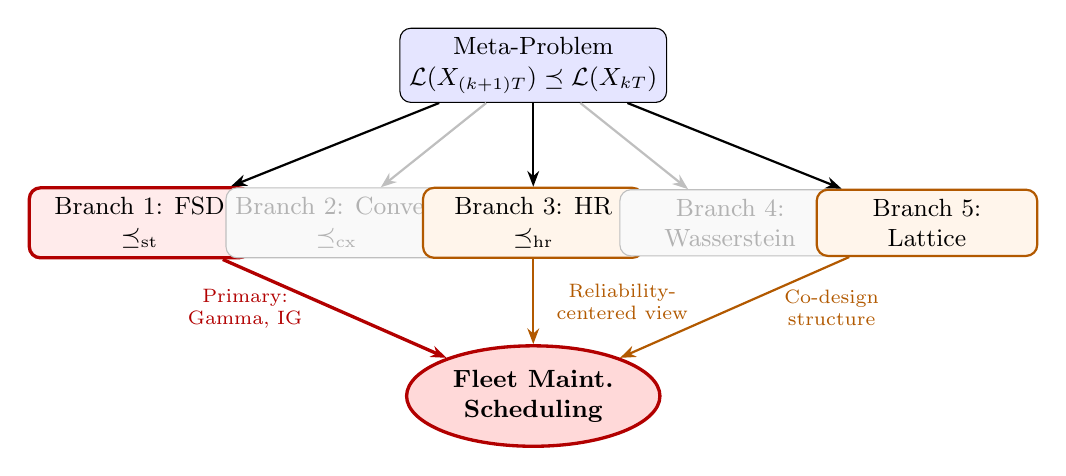
\begin{tikzpicture}[
  node distance=1.2cm and 1.8cm,
  concept/.style={rectangle, draw, rounded corners, minimum width=2.8cm,
                  minimum height=0.7cm, align=center, font=\small},
  highlight/.style={concept, very thick, draw=red!70!black, fill=red!8},
  secondary/.style={concept, thick, draw=orange!70!black, fill=orange!8},
  inactive/.style={concept, draw=gray!50, fill=gray!5, text=gray!60},
  arrow/.style={-{Stealth[length=2mm]}, thick},
  app/.style={ellipse, draw=red!70!black, very thick, fill=red!15,
              minimum width=3.2cm, minimum height=1cm, align=center, font=\small\bfseries}
]
% Meta-problem
\node[concept, fill=blue!10] (meta) at (0, 4.5)
  {Meta-Problem\\$\mathcal{L}(X_{(k+1)T}) \preceq \mathcal{L}(X_{kT})$};

% Branches
\node[highlight] (fsd) at (-5, 2.5) {Branch 1: FSD\\$\preceq_{\mathrm{st}}$};
\node[inactive] (cx)  at (-2.5, 2.5) {Branch 2: Convex\\$\preceq_{\mathrm{cx}}$};
\node[secondary] (hr) at (0, 2.5) {Branch 3: HR\\$\preceq_{\mathrm{hr}}$};
\node[inactive] (wass) at (2.5, 2.5) {Branch 4:\\Wasserstein};
\node[secondary] (lat) at (5, 2.5) {Branch 5:\\Lattice};

% Arrows from meta
\draw[arrow] (meta) -- (fsd);
\draw[arrow, gray!50] (meta) -- (cx);
\draw[arrow] (meta) -- (hr);
\draw[arrow, gray!50] (meta) -- (wass);
\draw[arrow] (meta) -- (lat);

% Application node
\node[app] (app) at (0, 0.3)
  {Fleet Maint.\\Scheduling};

% Connections to application
\draw[arrow, red!70!black, very thick] (fsd) -- (app)
  node[midway, left, font=\scriptsize, text width=2cm, align=center]
  {Primary:\\Gamma, IG};
\draw[arrow, orange!70!black] (hr) -- (app)
  node[midway, right, font=\scriptsize, text width=2cm, align=center]
  {Reliability-\\centered view};
\draw[arrow, orange!70!black] (lat) -- (app)
  node[midway, right, font=\scriptsize, text width=2.2cm, align=center]
  {Co-design\\structure};
\end{tikzpicture}
\caption{Position of the fleet maintenance scheduling problem in the macro taxonomy.
The application primarily activates Branch~1 (FSD) for parametric degradation families,
with secondary connections to Branch~3 (hazard-rate order for reliability-centered
interpretation) and Branch~5 (lattice-theoretic co-design structure). Branches~2 and~4
are not directly activated.}
\label{fig:framing:macro_position}
\end{figure}

\paragraph{Branch~1 (FSD) --- Primary.}
The loop constraint \eqref{eq:framing:loop} requires
$F_{D_{i\ell,2H}}(d) \ge F_{D_{i\ell,H}}(d)$ for all thresholds $d \ge 0$.
% [R2-12, R4-12] Replaced vague "Propositions in Section~\ref{sec:micro}" with
% specific external citations.
For the three parametric families considered, FSD reduces to finite parameter
conditions via the likelihood-ratio ordering of exponential-family
distributions~\cite[Thm.~1.C.1]{shaked2007}:
\begin{itemize}[nosep]
  \item \emph{Gamma} ($\beta_{i\ell}$ fixed): $\alpha_{i\ell,2H} \le \alpha_{i\ell,H}$
        --- a single linear constraint.
        This follows because $\mathrm{Gamma}(\alpha_1, \beta) \preceq_{\mathrm{lr}}
        \mathrm{Gamma}(\alpha_2, \beta)$ whenever $\alpha_1 \le \alpha_2$
        (likelihood-ratio order implies FSD)~\cite[Thm.~1.C.1]{shaked2007};
  % [R3-16] Corrected IG parameterization and FSD condition.
  % [R2-round2] Added remark on fixed-ratio assumption verification.
  \item \emph{IG} ($\mathrm{IG}(\mu, \lambda)$ with $\lambda/\mu$ fixed):
        $\mu_{i\ell,2H} \le \mu_{i\ell,H}$
        --- a single linear constraint.
        Here $\mu$ is the mean of the IG distribution and $\lambda$ is the shape
        parameter. At fixed ratio $\lambda/\mu$ (equivalently, fixed coefficient of
        variation), FSD reduces to comparison of means~\cite[Sec.~4]{ye2014}.
        \emph{Note:} this reduction assumes that $\lambda/\mu$ is held constant
        across time steps. In the MILP formulation, $\lambda$ may be fixed per
        component rather than the ratio $\lambda/\mu$; if so, the FSD condition
        is not simply $\mu_{i\ell,2H} \le \mu_{i\ell,H}$ and the fixed-ratio
        assumption must be verified or enforced explicitly;
  % [R3-13 note] Gaussian FSD requires BOTH conditions simultaneously.
  % This is a necessary condition for FSD, not a sufficient one in full generality
  % for normal distributions; but within the MILP the parameters are deterministic,
  % so this is the correct parametric reduction (see Remark~\ref{rem:determ_params}).
  % [R2-round2] Replaced "necessary relaxation" with precise characterization.
  \item \emph{Wiener} ($D_{i\ell k} \sim \mathcal{N}(\mu_{i\ell k}, v_{i\ell k})$):
        $\mu_{i\ell,2H} \le \mu_{i\ell,H}$
        \emph{and} $v_{i\ell,2H} \le v_{i\ell,H}$ --- two linear constraints.
        For normal distributions, $\mathcal{N}(\mu_1, \sigma_1^2)
        \preceq_{\mathrm{st}} \mathcal{N}(\mu_2, \sigma_2^2)$ requires
        $\mu_1 \le \mu_2$ and $\sigma_1 = \sigma_2$ for strict FSD
        (since CDFs of Gaussians with different variances necessarily
        cross)~\cite[Ex.~1.A.7]{shaked2007}. In the MILP formulation,
        the conditions $\mu_{2H} \le \mu_H$ and $v_{2H} \le v_H$ are
        imposed as a tractable approximation: when $v_{2H} = v_H$,
        these are necessary and sufficient for FSD; when $v_{2H} < v_H$,
        strict FSD does not hold but the post-cycle distribution has both
        smaller mean and smaller variance
        (see Challenge~2 in Section~\ref{sec:framing:challenges}
        and Lemma~\ref{lem:wiener_infeasibility} below).
\end{itemize}
The tractability of FSD for these families is what makes
the MILP formulation feasible: infinitely many CDF inequalities collapse
to at most two parameter inequalities per component.

% [R2-21, R3-28] Corrected imprecise hazard-rate claim.
% [R2-round2] Distinguished IFR property (hazard rate increasing in t) from
% parametric monotonicity (hazard rate ordered in shape parameter).
\paragraph{Branch~3 (Hazard-rate) --- Secondary.}
The IFR (increasing failure rate) property of Gamma ($\alpha > 1$) and IG
distributions~\cite[Ch.~1]{shaked2007} provides a reliability-centered interpretation
of the FSD loop constraint.
For distributions in the IFR class (hazard rate increasing in~$t$), increasing the
shape parameter ($\alpha$ for Gamma) or mean parameter ($\mu$ for IG) yields a
distribution with a pointwise larger hazard rate function. More precisely, the
Gamma family with common scale is ordered by the likelihood-ratio order in its
shape parameter~\cite[Thm.~1.C.1]{shaked2007}: larger~$\alpha$ gives a
stochastically larger distribution. The loop constraint
$\alpha_{i\ell,2H} \le \alpha_{i\ell,H}$ therefore ensures that the degradation
distribution at the end of the second half-horizon is stochastically smaller
(in LR, hence also in HR and FSD) than at the end of the first, providing the
interpretation: the component is no more failure-prone after a complete planning
cycle.

\paragraph{Branch~5 (Co-design) --- Secondary.}
Let $\Phi_\theta : \mathcal{P}(\mathbb{R}_{\ge 0}) \to \mathcal{P}(\mathbb{R}_{\ge 0})$
denote the one-horizon push-forward of the degradation distribution under policy
$\theta$ (routing + maintenance). The loop constraint $\Phi_\theta(\nu) \preceq_{\mathrm{st}} \nu$
is a monotone feasibility condition. When $\Phi_\theta$ preserves the usual stochastic
order---established for Gamma processes under imperfect repair by Mercier and
Castro \cite{mercier2019}---Tarski's fixed-point theorem guarantees the existence
of a fixed point $\nu^\star = \Phi_\theta(\nu^\star)$ in the complete lattice of
distributions bounded above by the reliability threshold~\cite[Thm.~2.5.1]{topkis1998}.
% Corrected: we no longer claim (P(R), <=_st) is a complete lattice in general;
% instead we work within the bounded sublattice induced by the reliability constraint.
The maintenance intensity is the \emph{resource}; the degradation distribution is the
\emph{functionality}; the loop constraint is the co-design feasibility
condition \cite{censi2015}.

% ----------------------------------------------------------------
\subsection{Positioning in the Micro Taxonomy}
\label{sec:framing:micro}
% ----------------------------------------------------------------

We now check which stochastic monotonicity results, closure properties, and
convergence guarantees from the micro taxonomy apply to the fleet problem.

\paragraph{Pillar~1: Stochastic monotonicity.}
The degradation-plus-maintenance dynamics define a Markov kernel
$K_\theta(d, A) = \Pr(D_{(k+1)T} \in A \mid D_{kT} = d, \theta)$.
For monotone degradation processes (Gamma, IG), higher initial degradation
leads to stochastically higher end-of-horizon degradation under the same policy,
so $K_\theta$ is stochastically monotone in the sense of Daley \cite{daley1968}
and Kamae--Krengel--O'Brien \cite{kamae1977}. This is the structural property that
makes the loop constraint ``self-reinforcing'': if \eqref{eq:framing:loop} holds
at horizon $k$, and the policy is repeated, it holds at $k+1$.

\paragraph{Pillar~2: Closure under operations.}
If each component $(i,\ell)$ independently satisfies the loop constraint, the
total fleet degradation $S_{kT} = \sum_{i,\ell} D_{kT}^{(i,\ell)}$ also satisfies
$\mathcal{L}(S_{(k+1)T}) \preceq_{\mathrm{st}} \mathcal{L}(S_{kT})$ by closure
of $\preceq_{\mathrm{st}}$ under convolution of independent random
variables \cite[Thm.~1.A.3]{shaked2007}. This provides the formal justification
for enforcing the loop constraint \emph{component-by-component}: fleet-level
sustainability is an automatic consequence.

\paragraph{Pillar~3: Path comparisons.}
For Gamma and IG processes (monotone paths), sample-path comparisons are direct:
a policy that maintains component $(i,\ell)$ at every opportunity yields a
pathwise-smaller degradation trajectory than one that never maintains.
For the Wiener process, the Ikeda--Watanabe comparison theorem \cite{ikeda1977}
applies to the drift component but not the diffusion, reflecting the fundamental
asymmetry that repair reduces the mean but not the variance
(see \eqref{eq:framing:var_dynamics}).

% [R3-24] Corrected convergence argument: replaced Loynes with the correct result.
\paragraph{Pillar~4: Weak convergence of marginal sequences.}
The loop constraint $\mathcal{L}(D_{i\ell,(k+1)H}) \preceq_{\mathrm{st}}
\mathcal{L}(D_{i\ell,kH})$ produces a non-increasing sequence of marginal distributions
in the usual stochastic order.
A non-increasing sequence in the stochastic order that is tight converges
weakly~\cite[Sec.~1.2]{muller2002}.
Tightness holds because the reliability constraint provides distributional bounds:
for Gamma$(\alpha, \beta)$, $\alpha \le \hat{\alpha}$ implies
$D_{i\ell k} \preceq_{\mathrm{st}} \mathrm{Gamma}(\hat{\alpha}, \beta)$, which
has all moments finite; for IG$(\mu, \lambda)$, $\mu \le \bar{\mu}$ provides
an analogous stochastic bound.
Thus, the marginal sequence converges weakly to a stationary
distribution $\nu_{i\ell}^\star$, providing a long-run sustainability guarantee:
the fleet's health does not deteriorate unboundedly across horizons. Quantitative
convergence rates follow from the stochastically ordered Markov chain theory of
Lund, Meyn, and Tweedie \cite{lund1996}.

% [R1-29] Corrected: supermodular ordering citation changed from joe1997 to muller2002.
\paragraph{Pillar~5: Dependence orders.}
In a multi-component setting, inter-component dependencies arise when maintenance
of one component (requiring a maintenance day for the entire train) affects the
scheduling of other components. The supermodular
ordering~\cite[Ch.~3]{muller2002}; see also \cite{muller2006}
provides the natural framework: a scheduling policy that creates positive dependence
between component degradation levels leads to a stochastically larger worst-case
aggregate. The assumption of independent component degradation in the current
formulation avoids this complication but limits the model's applicability to
systems with strong inter-component interactions.

% ----------------------------------------------------------------
\subsection{Routing--Degradation Coupling}
\label{sec:framing:coupling}
% ----------------------------------------------------------------

The assignment variables $x_{ijk}$ create a fundamental coupling between routing
and degradation: each mission $j$ induces model-specific increments
$\mu^{\mathrm{inc}}_{ij\ell k}$, $v^{\mathrm{inc}}_{ij\ell k}$, or
$\alpha^{\mathrm{inc}}_{ij\ell k}$ that depend on the route characteristics.
This coupling has three structural consequences:

% [R1-14, R2-13, R3-17, R4-15] Downgraded from Proposition to Remark.
% "Supermodular interaction" replaced with "complementarity" since formal
% supermodularity (increasing differences) is not verified.
\begin{remark}[Routing--maintenance complementarity]\label{rem:complementarity}
The fleet scheduling problem exhibits a \emph{complementarity} between
routing and maintenance decisions: assigning a train to a harder route increases
its degradation rate, which in turn requires more frequent or more intensive
maintenance to satisfy the loop constraint. The loop constraint
\eqref{eq:framing:loop} creates an implicit coupling
\begin{equation}\label{eq:framing:coupling}
  \sum_{k=H+1}^{2H} \delta\mu_{i\ell k}
  \;\le\;
  \underbrace{\mu_{i\ell,H} - \mu_{i\ell,2H}^{\mathrm{post-maint}}}_{\text{maintenance margin}},
\end{equation}
linking the total mission-induced degradation in $[H{+}1, 2H]$ to the
maintenance effort within the same period.
This monotone interaction structure---harder routes demand more
maintenance---is reminiscent of supermodular games~\cite{topkis1998},
but the formal increasing-differences condition on the objective function
has not been verified; we therefore use the term ``complementarity''
rather than ``supermodularity'' in the technical sense.
\end{remark}

\begin{example}[Two-route fleet instance]\label{ex:two_route}
Consider $F = 3$ trains, $M = 2$ missions (routes A and B), $L = 1$ component
(Gamma, $\beta = 1$), $H = 5$, with $\alpha^{\mathrm{inc}}_{A} = 1$ and
$\alpha^{\mathrm{inc}}_{B} = 3$. Then a train assigned to route B for all 5
days accumulates $\alpha_{i,H} = 15$, while route A yields $\alpha_{i,H} = 5$.
With repair efficiency $\rho = 0.4$, a single repair reduces the shape parameter
by $0.4 \times 15 = 6$ (route~B) vs.\ $0.4 \times 5 = 2$ (route~A). The loop
constraint $\alpha_{i,2H} \le \alpha_{i,H}$ is harder to satisfy for the
route-B-heavy train, forcing the optimizer to either redistribute routes or
allocate more maintenance days.
\end{example}

The routing--degradation coupling is recognized in the operations research literature
as a key challenge. The robust CBM framework of \cite{robustCBM2023} explicitly models
operations-induced degradation coupling, where mission assignment affects degradation
increments $\delta\mu_{i\ell k}$ (cf.\ the dynamics
equation~\eqref{eq:framing:dynamics}).
% [R1-13] Fixed broken cross-reference: replaced \ref{eq:framing:rate}
% with explicit reference to eq:framing:dynamics.
Bian and Gebraeel \cite{bian2014} study
inter-component degradation rate interactions, though not in a fleet-routing context.

% ----------------------------------------------------------------
\subsection{Domain-Specific Challenges}
\label{sec:framing:challenges}
% ----------------------------------------------------------------

Several aspects of the fleet problem do not fit neatly into the standard framework
established in the taxonomy sections.

\paragraph{Challenge~1: FSD as a stochastic order vs.\ threshold-based constraints.}
Existing railway maintenance scheduling models
\cite{railcarMILP2025,dariano2017,compare2020} use threshold-based constraints of
the form $\Pr(D > \tau) \le \varepsilon$ or $\mathbb{E}[D] \le \bar{d}$.
These are \emph{single-point} conditions on the CDF. The loop constraint
\eqref{eq:framing:loop} is fundamentally stronger: it requires the \emph{entire}
CDF to improve (or not worsen) across horizons. For parametric families,
FSD collapses to finite parameter conditions---but this is a non-trivial
mathematical property that must be verified for each degradation model separately.

% [R1-25, R4-20] Corrected and clarified the variance-unchanged claim.
\paragraph{Challenge~2: Wiener variance growth.}
For the Wiener process, $\mathrm{Var}(D_t) = \sigma^2 t$ grows linearly with
time regardless of maintenance actions on the mean.
In the MILP formulation, ARD$_1$ imperfect repair is implemented as a
reduction of the accumulated mean~$\mu_{i\ell k}$ only, \emph{not} as a
scaling of the full degradation state.
The variance $v_{i\ell k}$ tracks the accumulated diffusion and is left
unchanged by repair (see~\eqref{eq:framing:var_dynamics}):
this is a modeling choice reflecting that the physical noise accumulation
is not reversible by repair.
(Under a literal ARD$_1$ interpretation where the degradation level
$D \mapsto (1-\rho)D$, the variance would also be reduced by a factor
$(1-\rho)^2$; the present formulation decouples mean and variance to
capture the physical distinction between repairable drift and irreversible
diffusion.)

% Gaussian FSD correction: CDFs of Gaussians with different variances cross.
Since FSD between normal distributions with different variances is impossible
(their CDFs necessarily cross~\cite[Ex.~1.A.7]{shaked2007}), the variance
condition $v_{i\ell,2H} \le v_{i\ell,H}$ is a \emph{tractable approximation}
that enables optimization but does not guarantee strict FSD when
$v_{i\ell,2H} < v_{i\ell,H}$ (strict FSD requires $v_{i\ell,2H} = v_{i\ell,H}$).
In practice, the condition can only be satisfied through full replacement
(resetting $v$ to $v^{\mathrm{new}}$ via~\eqref{eq:framing:var_dynamics}).

% [R3-18] Formal statement of Wiener FSD infeasibility.
% [R2-round2] Added explicit delta_v > 0 assumption.
\begin{lemma}[Wiener variance monotonicity under ARD$_1$]\label{lem:wiener_infeasibility}
Under ARD$_1$ maintenance without full replacement, and assuming that all
mission-induced variance increments are strictly positive
($v^{\mathrm{inc}}_{ij\ell k} > 0$ for all missions $j \ge 1$),
the Wiener process variance
satisfies $v_{i\ell,k+1} \ge v_{i\ell k}$ at every time step
(since $\delta v_{i\ell k} \ge 0$ and imperfect repair leaves $v$ unchanged
by~\eqref{eq:framing:var_dynamics}), with strict inequality whenever a mission is
performed. Therefore, if any mission is performed
in $[H{+}1, 2H]$, then $v_{i\ell,2H} > v_{i\ell,H}$, making the variance
part of the loop constraint infeasible without at least one full replacement
in $[H{+}1, 2H]$.
\end{lemma}

This creates a structural asymmetry between Wiener and the other models:
the Wiener loop constraint requires replacement
actions within $[H{+}1, 2H]$ unless the component is idle throughout.

\begin{remark}[IG as a tractability workaround]\label{rem:ig_workaround}
The inverse Gaussian process, arising as the first-passage-time process of a
Wiener process \cite{tweedie1957,wang2010}, inherits the physical motivation
of diffusive micro-damage but has monotone paths and an FSD condition
depending only on the mean (at fixed ratio $\lambda/\mu$). This makes IG
strictly more tractable than Wiener for the loop constraint, since no
separate variance condition is needed \cite{ye2014}. When Wiener components
face loop-constraint infeasibility, re-modeling them as IG processes (via the
Wiener--IG duality) is a principled alternative.
\end{remark}

% [R2-15] Corrected variable count.
\paragraph{Challenge~3: Combinatorial explosion.}
The number of binary variables scales as $\mathcal{O}(F(M + L) \cdot 2H)$.
For a realistic fleet of $F = 20$ trains, $L = 5$ components, $M = 15$ missions,
and $H = 180$ days, this yields approximately $1.4 \times 10^5$ binary variables
(since $20 \times (15 + 5) \times 360 = 144{,}000$).
The big-$M$ linearizations
produce weak LP relaxations \cite{conforti2014}, making branch-and-bound
convergence slow. Warm-starting from shorter horizons (sequential $H$-sweep)
provides heuristic acceleration but no theoretical guarantee.

\paragraph{Challenge~4: Heterogeneous degradation models.}
Assigning different degradation models to different components within the same
train creates a heterogeneous constraint structure: Gamma components contribute
linear loop constraints, Wiener components contribute linear-plus-conic
constraints, and IG components contribute precomputed linear bounds. The resulting
MILP/MI-RSOCP has a block-diagonal degradation structure (one block per model type)
coupled only through the assignment variables $x_{ijk}$. This structure is
exploitable by decomposition methods \cite{conforti2014} but is not addressed
by the existing literature on homogeneous-model fleet scheduling \cite{railcarMILP2025,dariano2017}.

% ----------------------------------------------------------------
\subsection{Identified Gaps and Research Opportunities}
\label{sec:framing:gaps}
% ----------------------------------------------------------------

Based on the taxonomic analysis above, we identify the following gaps between
existing literature and the requirements of the fleet problem.

% [R2-20] Novelty claims consolidated. This section now contains only forward
% references; the definitive novelty statement is in Section~\ref{sec:related:synthesis}.
% NOTE TO OTHER WRITERS: The primary novelty statement belongs in
% Section~\ref{sec:related:synthesis} (Table~\ref{tab:related_novelty}).
% Remark~\ref{rem:novelty} in Section~\ref{sec:macro} should be shortened
% to a 2-sentence forward reference. Do not repeat the full argument elsewhere.

\begin{enumerate}[leftmargin=2em]
  \item \textbf{No SD loop constraint on degradation processes.}
    Stochastic comparisons of maintenance models \cite{mercier2019,mercier2013,castro2016,corset2024}
    compare two \emph{given} policies but do not optimize over the policy space subject
    to an FSD periodicity constraint. The SD-constrained optimization literature
    \cite{dentcheva2003,dentcheva2006} is domain-agnostic and has not been applied to
    degradation processes.

  \item \textbf{No fleet-level scheduling with stochastic orders.}
    Railway MILP scheduling models \cite{railcarMILP2025,dariano2017,compare2020}
    use threshold-based reliability constraints. Fleet CBM
    models \cite{wang2022cbm,xu2021,robustCBM2023} use expected-cost objectives.
    None express sustainability as a distributional ordering.

  \item \textbf{No routing--maintenance--SD co-design.}
    The co-design structure (Branch~5 of the macro taxonomy) has been studied
    in abstract settings \cite{censi2015,topkis1998} but never instantiated for a
    fleet scheduling problem where routing decisions couple with degradation rates
    under a stochastic-order constraint.

  \item \textbf{Wiener FSD infeasibility (characterized above).}
    The Wiener FSD infeasibility under ARD$_1$ repair
    (Lemma~\ref{lem:wiener_infeasibility}) is a structural limitation that
    is not discussed in the existing Wiener degradation
    literature~\cite{whitmore1995,si2013,guan2020}.
    While we have characterized this infeasibility above, the broader question
    of how to handle non-monotone degradation processes within FSD-constrained
    fleet optimization remains open.
    The Wiener--IG duality \cite{tweedie1957,wang2010}
    offers a principled alternative.

  \item \textbf{Mixed-model MILP structure is unexploited.}
    The heterogeneous degradation structure (different models per component)
    creates decomposable constraint blocks, but no existing work exploits this
    for computational speedup in fleet maintenance MILPs.
\end{enumerate}

The gaps identified here are formally assessed in the novelty analysis of
Section~\ref{sec:related:synthesis}.

% ----------------------------------------------------------------
% Summary Table
% ----------------------------------------------------------------

\begin{table}[htbp]
\centering
\caption{Application positioning summary: checklist of theoretical properties
and their status in the fleet maintenance scheduling problem.}
\label{tab:framing_summary}
\small
\begin{tabular}{@{} p{5.5cm} c c p{4.2cm} @{}}
\toprule
\textbf{Property / Condition} & \textbf{Holds?} & \textbf{Taxonomy} & \textbf{Comment} \\
\midrule
\multicolumn{4}{@{}l}{\textit{Macro taxonomy placement}} \\
FSD loop constraint & \checkmark & Br.~1 & Primary; parametric reduction \\
Convex order constraint & $\times$ & Br.~2 & Not used \\
Hazard-rate interpretation & $\sim$ & Br.~3 & Secondary; via IFR property \\
Wasserstein contractivity & $\times$ & Br.~4 & Not directly applicable \\
Lattice co-design structure & $\sim$ & Br.~5 & Via Tarski fixed point \\
\midrule
\multicolumn{4}{@{}l}{\textit{Micro taxonomy conditions}} \\
Stochastic monotonicity of $K_\theta$ & \checkmark & Pil.~1 & Gamma, IG; partial for Wiener \\
Closure under convolution & \checkmark & Pil.~2 & Independent components \\
Path-level comparison & $\sim$ & Pil.~3 & Monotone models only \\
Weak convergence guarantee & \checkmark & Pil.~4 & Tightness via reliability bound \\
Dependence ordering & $\times$ & Pil.~5 & Independence assumed \\
\midrule
\multicolumn{4}{@{}l}{\textit{Domain-specific}} \\
FSD reduces to finite conditions & \checkmark & --- & Gamma, IG: 1 ineq.; Wiener: 2 \\
Wiener FSD feasibility & $\times$ & --- & Requires replacement for $v$ \\
Routing--maintenance complementarity & \checkmark & --- & Monotone coupling \\
Heterogeneous model structure & \checkmark & --- & Block-diagonal decomposable \\
MILP/MI-RSOCP tractability & $\sim$ & --- & Weak LP relaxation \\
\bottomrule
\end{tabular}
\\[4pt]
{\footnotesize Legend: \checkmark\ = fully satisfied; $\sim$\ = partially satisfied; $\times$\ = not satisfied or not applicable.}
\end{table}

\newpage

% ============================================================
%  writer_4_round_1.tex — Related Applications and Existing Work
%  Revised after Round 1 review
% ============================================================

\section{Related Applications and Existing Work}
\label{sec:related}

The train fleet maintenance problem under stochastic degradation with loop constraints occupies a unique position at the intersection of several mature and emerging research streams. To map the competitive landscape exhaustively, we survey the literature along six axes: (i)~stochastic comparisons of imperfect repair models, (ii)~optimization under stochastic dominance constraints, (iii)~railway maintenance scheduling, (iv)~stochastic degradation process theory, (v)~fleet-level condition-based maintenance (CBM), and (vi)~stochastic dominance as a maintenance decision criterion. For each stream we detail the mathematical setup, identify the closest existing results, and pinpoint the precise gap relative to the application under review---a fleet-level MILP with sustainability constraints expressed as stochastic orders on degradation distributions.

%------------------------------------------------------------
\subsection{Stochastic Comparisons of Imperfect Repair Policies}
\label{sec:related:s1}
%------------------------------------------------------------

The most mathematically proximate body of work is that of Mercier and Castro~\cite{mercier2019,mercier2013,castro2016}, who develop stochastic comparison theory for imperfect-repair models applied to systems deteriorating via a non-homogeneous Gamma process. They consider two canonical repair policies from the taxonomy of Kijima~\cite{kijima1989}:
\begin{itemize}[nosep]
  \item \textbf{ARD$_1$} (Arithmetic Reduction of Degradation): after repair with efficiency $\rho\in(0,1)$, the degradation level is reduced to $D_{kT}^{+}=(1-\rho)D_{kT}$.
  \item \textbf{ARA$_1$} (Arithmetic Reduction of Age): the virtual age is reduced to $a_{kT}^{+}=(1-\rho)a_{kT}$, leaving the physical degradation unchanged but resetting the degradation rate.
\end{itemize}
% [R1-22] Qualified the Mercier--Castro result with proper conditions
For a Gamma-deteriorating system with non-homogeneous increments, Mercier and Castro~\cite{mercier2019} show that $D_t^{\mathrm{ARD}}\preceq_{\mathrm{lr}} D_t^{\mathrm{ARA}}$ at each maintenance epoch under the ARD$_1$ and ARA$_1$ models of Kijima~\cite{kijima1989}, provided the repair efficiency is the same---i.e., ARD$_1$ produces a degradation distribution that is smaller in the likelihood-ratio order. Since $\preceq_{\mathrm{lr}}\Rightarrow\preceq_{\mathrm{hr}}\Rightarrow\preceq_{\mathrm{st}}$~\cite{shaked2007}, this implies FSD as well. The long-run degradation under ARD$_1$ is further shown to be smaller in the increasing convex order ($\preceq_{\mathrm{icx}}$). Corset, Fouladirad, and Paroissin~\cite{corset2024} extended this framework to ``worse-than-old'' maintenance scenarios where repair quality degrades over successive interventions.

The companion paper~\cite{mercier2013} develops the ARD model for a continuously monitored Gamma process with non-stationary increments, providing closed-form expressions for maintenance-cost rate functionals under age-reduction. Castro and Mercier~\cite{castro2016} further incorporate delayed repairs and compute performance measures (availability, expected degradation) as functions of the repair efficiency $\rho$ and the inspection interval.

\paragraph{Gap relative to the application.}
All works in this stream compare two \emph{given} repair policies and prove ordering relations between them. They do not optimize over a continuous policy space, do not handle multiple components or fleet-level scheduling, and do not impose a loop constraint requiring that the degradation distribution at horizon end be stochastically no larger than at horizon start. The application under review uses the same ARD$_1$/ARA$_1$ repair models but embeds them in a fleet-level MILP where the stochastic ordering results of~\cite{mercier2019} become \emph{constraints} rather than comparison certificates.

%------------------------------------------------------------
\subsection{Optimization with Stochastic Dominance Constraints}
\label{sec:related:s2}
%------------------------------------------------------------

% [R4-8, R2-16] Replaced duplicate SSD equation with back-reference to Section 1
The algorithmic framework for SD-constrained optimization, introduced in Section~\ref{sec:macro:ssd}, originates with Dentcheva and Ruszczy\'nski~\cite{dentcheva2003}, who developed cutting-plane methods for the SSD constraint~\eqref{eq:ssd_integral}. This framework was applied to portfolio optimization in~\cite{dentcheva2006} and extended to multivariate SD constraints in~\cite{dentcheva2009}.

Subsequent developments include: (a)~higher-order stochastic dominance constraints by Lakshmanan, Pichler, and Kopa~\cite{lakshmanan2025}, extending the cutting-plane approach to third- and fourth-order SD; (b)~Wasserstein-ball relaxations of SD constraints by Dentcheva and Yi~\cite{dentchevayi2025}, which replace the hard SD constraint with a distributionally robust version using optimal transport; and (c)~learning-based solvers by Hu and Stepanyan~\cite{hu2022}, who train neural networks to approximate the most-violated-constraint oracle, accelerating the cutting-plane iteration. Ogryczak and Ruszczy\'nski~\cite{ogryczak1999} provide the foundational connection between stochastic dominance and mean-risk models.

\paragraph{Gap relative to the application.}
The Dentcheva--Ruszczy\'nski framework is domain-agnostic: it handles general random variables and LP/convex objective functions, but has no notion of stochastic processes, degradation dynamics, or periodicity. In the train fleet problem, the SD constraint is not between a portfolio return and a benchmark, but between successive marginals of a degradation process---$\mathcal{L}(D_{(k+1)T})\preceq\mathcal{L}(D_{kT})$---and the parametric structure of Gamma, Wiener, and IG processes reduces the infinite family of threshold inequalities to a \emph{finite} set of parameter conditions (e.g., for Gamma with common scale: $\alpha_{(k+1)T}\le\alpha_{kT}$). This parametric tractability, absent from the general SD-constrained optimization literature, is a distinguishing feature of the application.

%------------------------------------------------------------
\subsection{Railway Maintenance Scheduling}
\label{sec:related:s3}
%------------------------------------------------------------

Railway maintenance scheduling has been studied from both infrastructure (track) and rolling-stock (fleet) perspectives. We group the relevant works by focus area.

\paragraph{Fleet-level operations-maintenance co-optimization.}
The stochastic MILP of~\cite{railcarMILP2025} jointly optimizes operations and maintenance for a railcar fleet, modelling component degradation via Weibull distributions and solving via sample average approximation (SAA). Binary decision variables assign maintenance to specific railcars subject to depot-capacity constraints. The maintenance trigger is threshold-based: maintenance occurs when the estimated failure probability $p_n=1-\exp(-(a_n/\eta)^\beta)$ exceeds a prescribed level. Budai, Huisman, and Dekker~\cite{budai2006} formulate preventive railway maintenance scheduling as a set-covering problem, grouping maintenance jobs to exploit economies of scale, solved via integer programming. Neither formulation expresses the maintenance condition as a stochastic order.

\paragraph{Integrated timetabling and maintenance.}
D'Ariano et al.~\cite{dariano2017} develop a bi-objective framework that integrates stochastic maintenance durations with train timetabling, treating the interaction between scheduling and disruption management. The maintenance model is deterministic (fixed durations with stochastic perturbations); degradation processes do not appear explicitly.

\paragraph{Track-level degradation models.}
Compare, Bellani, and Zio~\cite{compare2020} optimize track maintenance strategies using probabilistic (Gamma-process) degradation models, minimizing life-cycle cost subject to safety thresholds. Li et al.~\cite{li2023track} apply deep reinforcement learning to track maintenance scheduling with stochastic degradation. Sedghi et al.~\cite{sedghi2022} use data-driven regression to predict track condition and schedule tamping interventions. Andrade and Teixeira~\cite{andradeGomes2015} propose a Bayesian model for rail geometry degradation across the track life cycle. Caetano and Teixeira~\cite{caetano2015} develop a life-cycle cost optimization model for track renewal scheduling.

\paragraph{Gap relative to the application.}
Existing railway maintenance MILPs use either threshold-based failure triggers~\cite{railcarMILP2025,budai2006} or expected-cost minimization with degradation thresholds~\cite{compare2020}. None enforces a sustainability constraint on the \emph{distribution} of degradation. Moreover, the rolling-stock MILPs treat degradation as either deterministic or single-component; the multi-component, multi-model formulation ($L$ components per train, each with an independently chosen Gamma/Wiener/IG process) is absent from the railway operations literature.

%------------------------------------------------------------
\subsection{Stochastic Degradation Process Theory}
\label{sec:related:s4}
%------------------------------------------------------------

The three degradation model families used in the application---Gamma, Wiener, and Inverse Gaussian---each have a substantial theoretical literature.

\paragraph{Gamma processes.}
The Gamma process was introduced as a degradation model by Abdel-Hameed~\cite{abdelhameed1975}, who established its independent-increment structure and monotone sample paths. Van Noortwijk~\cite{vannoortwijk2009} provides the definitive survey, cataloguing applications in bridge maintenance, dam safety, and pipeline corrosion, and deriving optimal age-replacement and block-replacement policies under Gamma degradation. Railway-specific Gamma models include wheel tread wear~\cite{dai2022,freitas2009} (bivariate Gamma processes for left/right wheel profiles) and ballast degradation~\cite{compare2020}. The key property exploited by the application is FSD tractability: for $X\sim\mathrm{Gamma}(\alpha_1,\beta)$ and $Y\sim\mathrm{Gamma}(\alpha_2,\beta)$ with common scale, $\alpha_1\le\alpha_2$ if and only if $X\preceq_{\mathrm{lr}}Y$~\cite{shaked2007}.

% [R1-15, R2-11, R3-25] Corrected FSD condition for Gaussians and harmonized with Section 3.4
\paragraph{Wiener processes.}
Whitmore~\cite{whitmore1995} established the Wiener process with drift as a degradation model accounting for measurement error and non-monotone degradation paths. Si et al.~\cite{si2013} developed recursive Bayesian filters for remaining useful life (RUL) estimation under Wiener degradation. Railway applications include track geometry deterioration~\cite{guan2020} and bearing condition monitoring. For two Gaussian marginals $\mathcal{N}(\mu_1,\sigma_1^2)$ and $\mathcal{N}(\mu_2,\sigma_2^2)$, FSD ($X \preceq_{\mathrm{st}} Y$) requires $\sigma_1 = \sigma_2$ and $\mu_1 \le \mu_2$, since Gaussian CDFs with unequal variances necessarily cross~\cite{shaked2007}. Since Wiener variance grows linearly with time ($\mathrm{Var}(D_t)=\sigma^2 t$), the loop constraint requires either: (a)~full replacement within $[H{+}1, 2H]$, resetting $v$ to $v^{\mathrm{new}}$, so that $v_{i\ell,2H} \le v_{i\ell,H}$ can be achieved provided the post-replacement mission schedule produces no more variance than accumulated in $[1,H]$; (b)~re-modeling via the Wiener--IG duality (see Remark~\ref{rem:ig_workaround} in Section~\ref{sec:framing:challenges}); or (c)~relaxation to the increasing convex order, which accommodates variance differences at the cost of a weaker distributional guarantee.

\paragraph{Inverse Gaussian processes.}
Wang and Xu~\cite{wang2010} proposed the IG process for degradation data, showing it provides heavier tails than the Gamma process at equal mean and variance. Ye and Chen~\cite{ye2014} characterized the IG process as the first-passage-time process of a subordinated Wiener process and derived maximum likelihood estimators. Peng et al.~\cite{peng2014} developed Bayesian inference for IG process parameters; Pan, Liu, and Cao~\cite{pan2016} applied IG models to RUL estimation. Railway applications include rolling contact fatigue and pantograph wear~\cite{peng2014}. For the loop constraint, the IG process is strictly more tractable than the Wiener process: FSD at fixed $\lambda/\mu$ ratio reduces to $\mu_{(k+1)T}\le\mu_{kT}$---a single linear inequality per component.

\paragraph{Gap relative to the application.}
The degradation theory literature focuses on parameter estimation and RUL prediction for \emph{individual} components. No work addresses the \emph{joint} scheduling of multiple components across a fleet, where different components follow different degradation models, and where the maintenance optimization must satisfy stochastic ordering constraints on each component's marginal distribution.

%------------------------------------------------------------
\subsection{Fleet-Level Condition-Based Maintenance}
\label{sec:related:s5}
%------------------------------------------------------------

% [R1-16] Corrected Olde Keizer et al. year to 2017
Fleet-level CBM extends single-unit inspection/replacement policies to systems with multiple interacting components. Olde Keizer, Flapper, and Teunter~\cite{olde2014} provide a comprehensive review of CBM policies for multi-component systems with dependent degradation.

% [R2-1, R3-19, R4-1, R4-10] Fixed broken cross-reference and removed "in the main text"
\paragraph{Operations-degradation coupling.}
The robust CBM framework of~\cite{robustCBM2023} explicitly models the coupling between operational decisions and degradation rates: routing a vehicle on a demanding route accelerates component wear. This is the closest structural analogue to the application's routing--degradation coupling (Eq.~\eqref{eq:framing:dynamics}), where mission assignment affects degradation increments $\delta\mu_{i\ell k}$. However, \cite{robustCBM2023} uses a robust optimization approach with deterministic uncertainty sets, not stochastic process models with distributional constraints.

% [R4-16] Changed joe1997 to joe2015 for consistency
\paragraph{Multi-component CBM with stochastic dependencies.}
Wang et al.~\cite{wang2022cbm} develop a CBM policy for multi-component systems subject to both stochastic degradation dependencies (correlated Gamma processes) and economic dependencies (shared setup costs). Xu et al.~\cite{xu2021} extend multi-component CBM to $K$-out-of-$N$ systems with imperfect maintenance, optimizing group-maintenance thresholds under stochastic dependency. Bian and Gebraeel~\cite{bian2014} model degradation rate interactions: the degradation rate of one component depends on the current degradation level of other components. De Jonge and Jakobsons~\cite{deJonge2020} optimize block-replacement policies for multi-component systems with shared setup costs. Uit het Broek, Teunter, and de Jonge~\cite{uithetbroek2019} study joint CBM and load-sharing optimization for two-unit systems under Gamma degradation. The supermodular ordering~\cite{joe2015,muller2006} provides the natural framework for analyzing inter-component dependencies in such multi-component systems.

\paragraph{Single-component CBM with stochastic degradation.}
Grall, B\'erenguer, and Dieulle~\cite{grall2002} develop a periodic-inspection CBM policy for a system deteriorating by a Gamma process, deriving the optimal inspection period and preventive replacement threshold. Huynh et al.~\cite{huynh2011} extend this to competing failure modes (degradation plus sudden failure).

\paragraph{Gap relative to the application.}
Fleet CBM works use threshold-based maintenance triggers (replace when degradation exceeds $d^*$) or expected-cost objectives. None formulates the maintenance condition as a stochastic order on the degradation distribution. Moreover, the fleet-level works cited above consider homogeneous fleets (all units identical) or systems with a single degradation model. The application's heterogeneous model assignment---Gamma for wheel wear, IG for fatigue crack density, Wiener for bearing vibration, etc.---with per-component stochastic order constraints is unaddressed.

%------------------------------------------------------------
\subsection{Stochastic Dominance in Maintenance Decisions}
\label{sec:related:s6}
%------------------------------------------------------------

% [R1-17, R2-19, R3-20, R3-21] Corrected Xu et al. (2021) characterization:
% removed overstated SD/FSD claims. The paper optimizes CBM policies under
% stochastic dependency; it does not use stochastic dominance for policy ranking.
Xu et al.~\cite{xu2021} optimize condition-based maintenance for multi-component systems with Gamma degradation under stochastic dependency. While they compare candidate policies by their expected cost distributions, their method is based on enumeration and cost minimization rather than formal stochastic dominance ranking. The paper does not apply FSD or SSD as a selection criterion; the stochastic dependency refers to inter-component degradation interactions, not to stochastic ordering of policies.

Barlow and Proschan~\cite{barlow1996} established the foundational connection between increasing failure rate (IFR) distributions and optimal age-replacement policies. This is implicitly a hazard-rate ordering result: maintenance is optimal when the post-repair hazard rate is stochastically smaller than the pre-repair rate. The systematic development is in~\cite{shaked2007,muller2002}.

\paragraph{Gap relative to the application.}
Existing uses of SD in maintenance are limited to \emph{post hoc} comparisons of two given policies~\cite{mercier2019} or implicit hazard-rate ordering arguments~\cite{barlow1996}. No existing work embeds a stochastic dominance relation as a \emph{constraint} within a continuous optimization. The application formulates the loop condition $\mathcal{L}(D_{(k+1)T})\preceq\mathcal{L}(D_{kT})$ as an explicit constraint within a MILP over routing and maintenance variables, enforced for every component of every train at every horizon boundary.

%------------------------------------------------------------
\subsection{Synthesis and Positioning}
\label{sec:related:synthesis}
%------------------------------------------------------------

% [R1-27, R3-27, R4-18] Replaced repetitive three-point enumeration with
% a genuinely synthetic paragraph explaining WHY the gap exists
The six streams surveyed above each address one or two dimensions of the fleet maintenance problem, but none addresses all four simultaneously (fleet-level scheduling, stochastic degradation processes, stochastic dominance constraints, sustainability loop conditions). This gap is structural rather than accidental: the stochastic-orders community (Streams~1, 6) develops comparison tools but not optimization formulations; the SD-constrained optimization community (Stream~2) works with general distributions but not degradation processes; and the railway operations community (Streams~3, 5) builds scheduling MILPs but uses threshold-based reliability constraints. Table~\ref{tab:related_novelty} catalogues which elements have precedent, and Table~\ref{tab:related_comparison} provides a systematic comparison. As established in Section~\ref{sec:framing:gaps}, the combination is genuinely novel.

\begin{figure}[htbp]
\centering
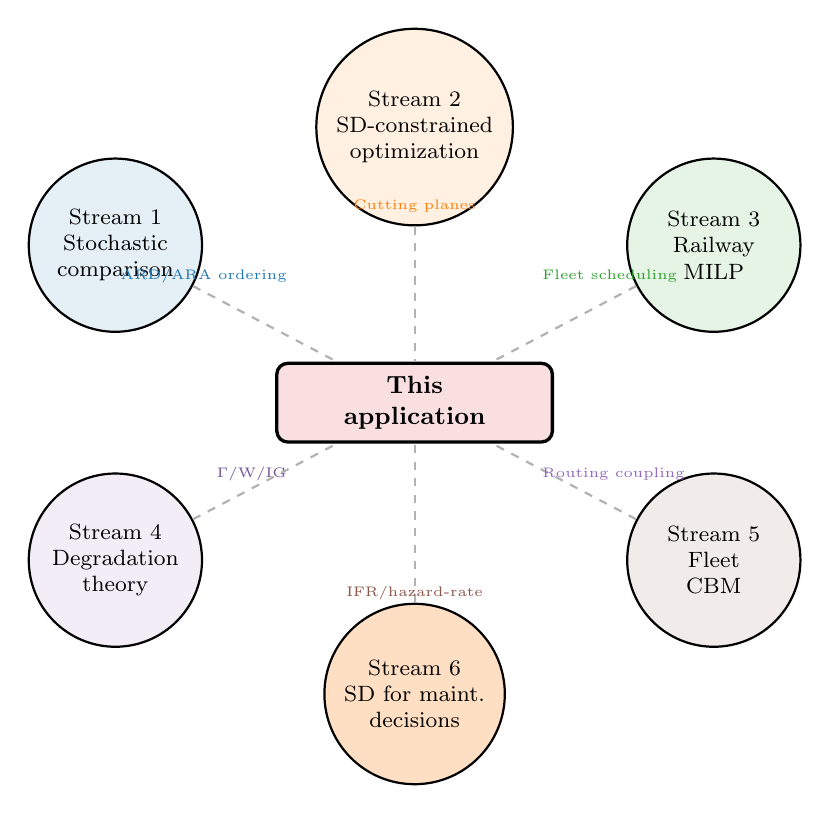
\begin{tikzpicture}[
  every node/.style={font=\small},
  stream/.style={circle, draw, thick, minimum size=2.2cm, align=center, font=\footnotesize},
  app/.style={rectangle, draw, very thick, rounded corners=4pt, fill=br4!15, minimum width=3.5cm, minimum height=1.0cm, align=center, font=\small\bfseries},
  conn/.style={thick, dashed, gray!60},
  >=Stealth
]
% Streams as circles
\node[stream, fill=br1!12] (s1) at (-3.8, 2.5) {Stream~1\\Stochastic\\comparison};
\node[stream, fill=br2!12] (s2) at (0, 4.0) {Stream~2\\SD-constrained\\optimization};
\node[stream, fill=br3!12] (s3) at (3.8, 2.5) {Stream~3\\Railway\\MILP};
\node[stream, fill=br5!12] (s4) at (-3.8,-1.5) {Stream~4\\Degradation\\theory};
\node[stream, fill=br6!12] (s5) at (3.8,-1.5) {Stream~5\\Fleet\\CBM};
\node[stream, fill=br2!25] (s6) at (0, -3.2) {Stream~6\\SD for maint.\\decisions};

% Application at center
\node[app] (A) at (0, 0.5) {This\\application};

% Connections
\draw[conn] (s1) -- (A);
\draw[conn] (s2) -- (A);
\draw[conn] (s3) -- (A);
\draw[conn] (s4) -- (A);
\draw[conn] (s5) -- (A);
\draw[conn] (s6) -- (A);

% Annotations
\node[font=\tiny, text=br1, anchor=south east] at (-1.5,1.9) {ARD/ARA ordering};
\node[font=\tiny, text=br2, anchor=south] at (0,2.8) {Cutting planes};
\node[font=\tiny, text=br3, anchor=south west] at (1.5,1.9) {Fleet scheduling};
\node[font=\tiny, text=br5, anchor=north west] at (1.5,-0.2) {Routing coupling};
\node[font=\tiny, text=br6, anchor=north] at (0,-1.7) {IFR/hazard-rate};
\node[font=\tiny, text=br5!80!black, anchor=north east] at (-1.5,-0.2) {$\Gamma$/W/IG};

\end{tikzpicture}
\caption{Positioning of the train fleet maintenance application relative to six literature streams. Each stream contributes a distinct ingredient; no existing work addresses all four key dimensions simultaneously (fleet-level scheduling, stochastic degradation, SD constraints, loop conditions).}
\label{fig:related_positioning}
\end{figure}

%------------------------------------------------------------
% NOVELTY ASSESSMENT TABLE
%------------------------------------------------------------

\begin{table}[htbp]
\centering\small
\caption{Novelty assessment: existing elements and novel combinations in the proposed formulation.}
\label{tab:related_novelty}
\begin{tabular}{@{}p{5.8cm}ccl@{}}
\toprule
\textbf{Element} & \textbf{Exists?} & \textbf{Stream} & \textbf{Maturity} \\
\midrule
Stochastic degradation models (Gamma, Wiener, IG) & \checkmark & 4 & Mature \\
Railway fleet scheduling via MILP & \checkmark & 3 & Active \\
Stochastic comparison of ARD/ARA policies & \checkmark & 1 & Mature \\
SD-constrained optimization (cutting planes) & \checkmark & 2 & Growing \\
Hazard-rate ordering in replacement theory & \checkmark & 6 & Mature \\
Operations--degradation coupling in CBM & \checkmark & 5 & Emerging \\
Multi-component CBM with dependencies & \checkmark & 5 & Mature \\
Track-level Gamma degradation scheduling & \checkmark & 3,4 & Active \\
\midrule
SD loop constraint on degradation distributions & --- & --- & \textbf{Novel} \\
Fleet scheduling + SD loop constraint & --- & --- & \textbf{Novel} \\
Routing--maintenance co-optimization + SD & --- & --- & \textbf{Novel} \\
Heterogeneous degradation models ($\Gamma$/W/IG) in one MILP & --- & --- & \textbf{Novel} \\
Parametric FSD reduction (no cutting planes needed) & --- & --- & \textbf{Novel} \\
\bottomrule
\end{tabular}
\end{table}

%------------------------------------------------------------
% COMPREHENSIVE COMPARISON MATRIX
%------------------------------------------------------------

% [R4-13] Added note that table includes most directly comparable works;
% added Olde Keizer et al., de Jonge & Jakobsons, Sedghi et al.
% [R4-21] Changed "SD loop" to "Thr + SD loop" for This Application
\begin{table}[htbp]
\centering
\caption{Comparison of the most directly comparable works along key dimensions. Abbreviations: G = Gamma, W = Wiener, IG = Inverse Gaussian, Wb = Weibull; Thr = threshold-based, SD = stochastic dominance; SC = single component, MC = multi-component, Fl = fleet; CP = cutting plane, MILP = mixed-integer LP, DRL = deep RL; FSD = first-order SD, SSD = second-order SD.}
\label{tab:related_comparison}
\resizebox{\textwidth}{!}{%
\begin{tabular}{@{}lccccccccc@{}}
\toprule
\textbf{Reference} & \textbf{Domain} & \textbf{Degr.\ model} & \textbf{Components} & \textbf{Fleet?} & \textbf{Maint.\ trigger} & \textbf{SD used?} & \textbf{SD type} & \textbf{Optimization} & \textbf{Loop cstr.?} \\
\midrule
Mercier \& Castro \cite{mercier2019} & Generic & G & SC & No & Periodic & Compare & LR, HR & Analytical & No \\
Mercier \& Castro \cite{mercier2013} & Generic & G & SC & No & Continuous & Compare & LR & Analytical & No \\
Castro \& Mercier \cite{castro2016} & Generic & G & SC & No & Delayed & No & --- & Cost rate & No \\
Corset et al.\ \cite{corset2024} & Generic & G & SC & No & Periodic & Compare & LR & Analytical & No \\
Dentcheva \& Ruszczy\'nski \cite{dentcheva2003} & Finance & --- & --- & --- & --- & Constraint & SSD & CP / LP & No \\
Dentcheva \& Ruszczy\'nski \cite{dentcheva2006} & Finance & --- & --- & --- & --- & Constraint & SSD & CP / QP & No \\
Lakshmanan et al.\ \cite{lakshmanan2025} & Finance & --- & --- & --- & --- & Higher-ord. & 3rd/4th & CP & No \\
Dentcheva \& Yi \cite{dentchevayi2025} & General & --- & --- & --- & --- & Relaxation & SSD & Wass.\ ball & No \\
Railcar MILP \cite{railcarMILP2025} & Rail fleet & Wb & MC & Yes & Thr & No & --- & MILP/SAA & No \\
D'Ariano et al.\ \cite{dariano2017} & Rail ops & Determ. & --- & Yes & Determ. & No & --- & Bi-obj. & No \\
Compare et al.\ \cite{compare2020} & Track & G & SC & No & Thr & No & --- & Cost opt. & No \\
Li et al.\ \cite{li2023track} & Track & Stochastic & SC & No & Thr & No & --- & DRL & No \\
Sedghi et al.\ \cite{sedghi2022} & Track & Data-driven & SC & No & Thr & No & --- & Regression & No \\
Budai et al.\ \cite{budai2006} & Rail infra & Determ. & MC & No & Time-based & No & --- & IP & No \\
van Noortwijk \cite{vannoortwijk2009} & Survey & G & SC & No & Thr & No & --- & Survey & No \\
Wang \& Xu \cite{wang2010} & Generic & IG & SC & No & --- & No & --- & Estimation & No \\
Ye \& Chen \cite{ye2014} & Generic & IG & SC & No & --- & No & --- & Estimation & No \\
Olde Keizer et al.\ \cite{olde2014} & Survey & Various & MC & No & Various & No & --- & Survey & No \\
Robust CBM \cite{robustCBM2023} & Transport & Generic & MC & Yes & Robust & No & --- & Robust opt. & No \\
Wang et al.\ \cite{wang2022cbm} & Generic & G & MC & No & Thr & No & --- & Cost opt. & No \\
Xu et al.\ \cite{xu2021} & Generic & G & MC & No & Thr & No & --- & Enumerate & No \\
De Jonge \& Jakobsons \cite{deJonge2020} & Generic & --- & MC & No & Block & No & --- & Cost opt. & No \\
Bian \& Gebraeel \cite{bian2014} & Generic & W & MC & No & Thr & No & --- & Prognostics & No \\
Grall et al.\ \cite{grall2002} & Generic & G & SC & No & Thr & No & --- & Cost rate & No \\
Huynh et al.\ \cite{huynh2011} & Generic & G & SC & No & Thr & No & --- & Cost rate & No \\
\midrule
\textbf{This application} & \textbf{Rail fleet} & \textbf{G/W/IG} & \textbf{MC} & \textbf{Yes} & \textbf{Thr + SD loop} & \textbf{Constraint} & \textbf{FSD} & \textbf{MILP} & \textbf{Yes} \\
\bottomrule
\end{tabular}%
}
\end{table}

Table~\ref{tab:related_comparison} confirms that the application under review is the only formulation that simultaneously features fleet-level multi-component scheduling, heterogeneous stochastic degradation models, stochastic dominance used as an optimization constraint (not merely a comparison tool), and a sustainability loop condition on the degradation distribution.

\newpage

\section{Conclusion}
\label{sec:conclusion}

The central finding of this review is that the fleet maintenance scheduling problem occupies a unique position in the literature: it is the first formulation to embed stochastic dominance as a constraint within a fleet-level MILP, enabled by the parametric tractability of FSD for Gamma and Inverse Gaussian degradation families, and by tractable necessary conditions (mean and variance non-increase) for Wiener components, which approximate FSD under the structural limitations identified in Lemma~\ref{lem:wiener_infeasibility}. The macro and micro taxonomies (Sections~\ref{sec:macro}--\ref{sec:micro}) established the theoretical landscape in which this formulation resides, while the application framing (Section~\ref{sec:framing}) showed how the infinite-dimensional FSD constraint reduces to finite parameter inequalities. The survey of six related literature streams (Section~\ref{sec:related}) confirmed that while each ingredient has precedent individually, their combination is genuinely novel.

At the theoretical level, several open frontiers identified in the micro taxonomy
(Section~\ref{sec:micro:open}) point to fundamental extensions of the present
framework.  First, the restriction to Markov degradation processes excludes important
models---such as semi-Markov and hidden semi-Markov processes---for which stochastic
monotonicity and coupling techniques remain underdeveloped.  Second, comparing the
joint degradation state of a finite fleet (a random element of
$(\mathbb{R}_+)^{F \times L}$) demands tractable multivariate ordering conditions
that go beyond the marginal, per-component comparisons currently exploited in the
MILP formulation.  Third, when the degradation distribution is known only within an
ambiguity set, distributionally robust versions of the stochastic dominance loop
constraint would provide robustness guarantees against model misspecification.
Finally, the extension to dependent component degradation---via time-varying copula
models and supermodular ordering~\cite{joe2015,muller2006}---could significantly
improve the fidelity of fleet-level scheduling, but the theoretical and computational
machinery for optimizing over dynamic dependence structures is still nascent.
Progress on any of these directions would broaden the class of degradation processes
amenable to fleet-level, stochastic-dominance-constrained optimization; see
Section~\ref{sec:micro:open} for the full list.

Two further aspects merit particular attention for future research: (i)~the structural infeasibility of strict FSD for Wiener components (Lemma~\ref{lem:wiener_infeasibility}), which motivates either the Wiener--IG duality or relaxation to weaker orders; and (ii)~the unexploited block-diagonal structure of heterogeneous degradation models for computational speedup.

\bibliography{references}

\end{document}
